\documentclass[11pt]{article}
\usepackage{geometry}
\geometry{
 a4paper,
 total={210mm,297mm},
 left=20mm,
 right=20mm,
 top=20mm,
 bottom=20mm,
 }
 
\usepackage[english]{babel}
\usepackage[utf8x]{inputenc}
\usepackage{amsmath}
\usepackage{graphicx}
\usepackage[table,xcdraw]{xcolor}
\usepackage[colorinlistoftodos]{todonotes}
\usepackage{multicol}
\usepackage{ragged2e}
\usepackage{tocloft}
\usepackage{titlesec}
\usepackage{natbib}
\usepackage[parfill]{parskip}
\usepackage{amssymb}
\usepackage{textcomp}
\usepackage{float}
\floatstyle{plain}
\usepackage{color}
\usepackage{epstopdf}
\usepackage{hyperref}
\usepackage{comment}
\hypersetup{
    colorlinks=true,
    linkcolor=blue,
    filecolor=magenta,      
    urlcolor=cyan,
    citecolor=blue
}
\urlstyle{same}
\usepackage{fancyhdr}
\usepackage{lipsum}
\usepackage{subscript}
\usepackage{siunitx}
\usepackage[hypcap]{caption}
\usepackage{capt-of}
\usepackage{wasysym}
\usepackage{wrapfig}
\usepackage{enumitem}
\usepackage{pdflscape}
\usepackage{pdfpages}
\usepackage{csquotes}
\usepackage{mathtools}

%making the bloody title 
\makeatletter
\renewcommand{\maketitle}{\bgroup\setlength{\parindent}{0pt}
\begin{flushleft}
  \textbf{\@title} %the empty line is impt

  \@author
\end{flushleft}\egroup
}
\makeatother

%random things needed
%\renewcommand{\cftsecleader}{\cftdotfill{\cftdotsep}} %let the content table have dots to number
\linespread{1.5}  %making one and a half spacing-sh one and half is actually 1.3
\frenchspacing
%\titlespacing\subsection{0pt}{12pt plus 4pt minus 2pt}{0pt plus 2pt minus 2pt} 
\titlespacing\subsubsection{0pt}{12pt plus 4pt minus 2pt}{0pt plus 2pt minus 2pt} %less spacing between subsubsections
\pagestyle{fancy}
% Set the right side of the footer to be the page number
\fancyhf{} % sets both header and footer to nothing
\renewcommand{\headrulewidth}{0pt}
\fancyfoot[R]{\thepage}
\fancypagestyle{plain}{%
    \renewcommand{\headrulewidth}{0pt}%
    \fancyhf{}%
    \fancyfoot[R]{\thepage}%
}
\setlength{\parskip}{0pt}
%make modulus same length as text, starred makes it shorter
\DeclarePairedDelimiter\abs{\lvert}{\rvert}%
\DeclarePairedDelimiter\norm{\lVert}{\rVert}%

%insert title
\title{\textbf{\LARGE{Skeleton}}}
\smallskip
\date{} 
\author{%
\large{Lim Jia Le}
}

\begin{document}
\maketitle
\smallskip
\tableofcontents

% word limit 6000 words

\section{Introduction} % 800 words
What is a network? \\
What is turnover? \\
Previous studies \\
Why study turnover? \\
Why is it important to know climate impacts on turnover? \\
Why pollinator, why bees ? \\
Flowchart \\
short summary of paper \& results \\

\section{Methods} % 1500 words
Two datasets. How data was collected?\\
Climate data from? \\
Why use $\beta$-dissimilarity measure? \\
Explain $\beta$-dissimilarity measure? \\
How the different turnover measures are calculated - use table \\
why use sum of precipitation, the rest medians used due to skrewed distributions. \\
why do not use humidity, only use avg temps \\
two climate models, test to see which climate model is better \\
Model fitting\\
Why use spearman to calculate correlation \\
Use Randomization/Monte Carlo to check p-value to show results correlation not random \\
Does not correlate with p-values due to datapoints not being independent of each other\\
How Monte Carlo was simulated \\

\section{Results} % 1800 words
Abundance of bees, plants in both sites \\
Amt of data points, amount of interactions, amount of unique interactions \\
Small sample size , use randomization to reduce sample bias, show that p-values of spearman test does not correspond with p-values generated from MonteCarlo \\
High turnover\\
\\
\underline{Bbee correlates with Bplant} \\
Low correlation in Cerrado (2008-2009) Dry Season, probably due to outlier and few data points.\\

\begin{figure}[H]
\makebox[\textwidth]{%
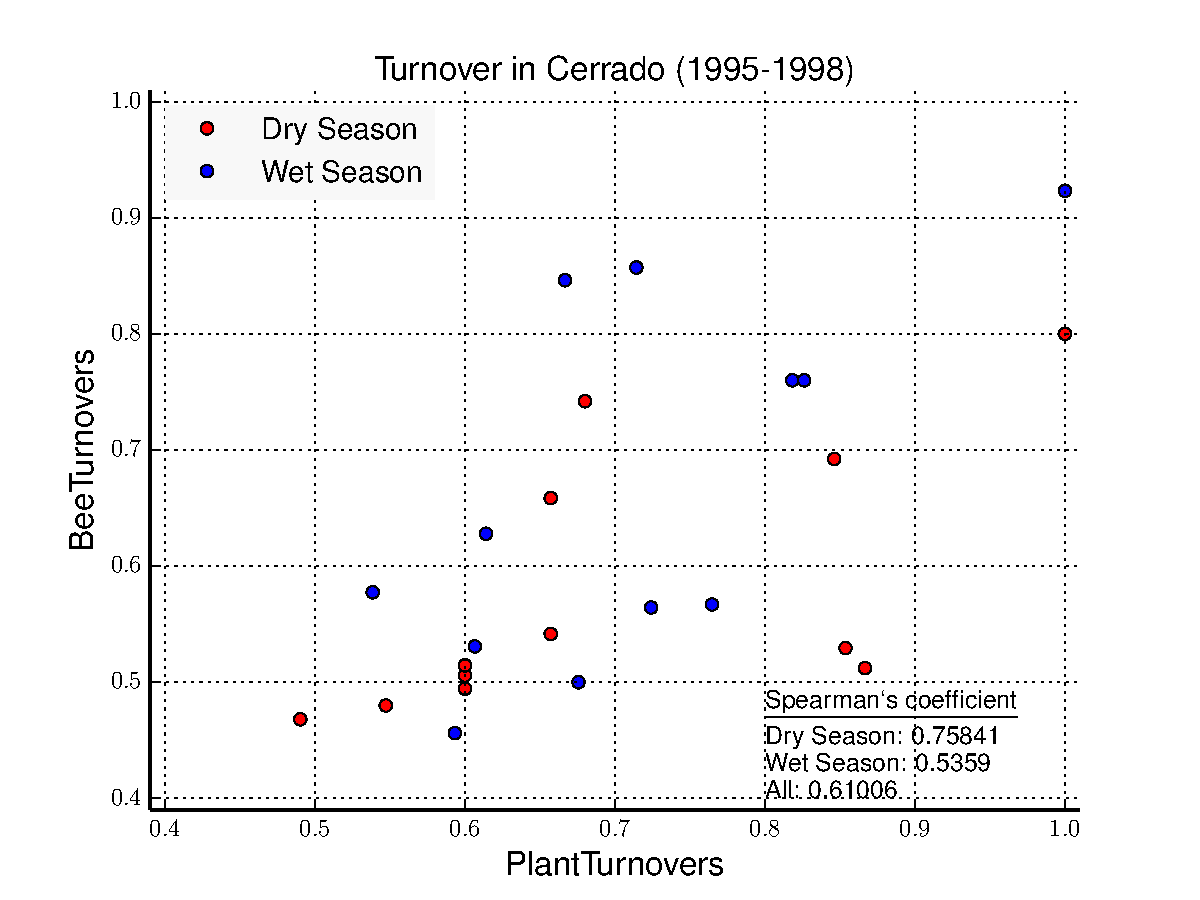
\includegraphics[width=0.48\textwidth]{PlantTurnovers-BeeTurnovers(old).pdf}%
\hfill    
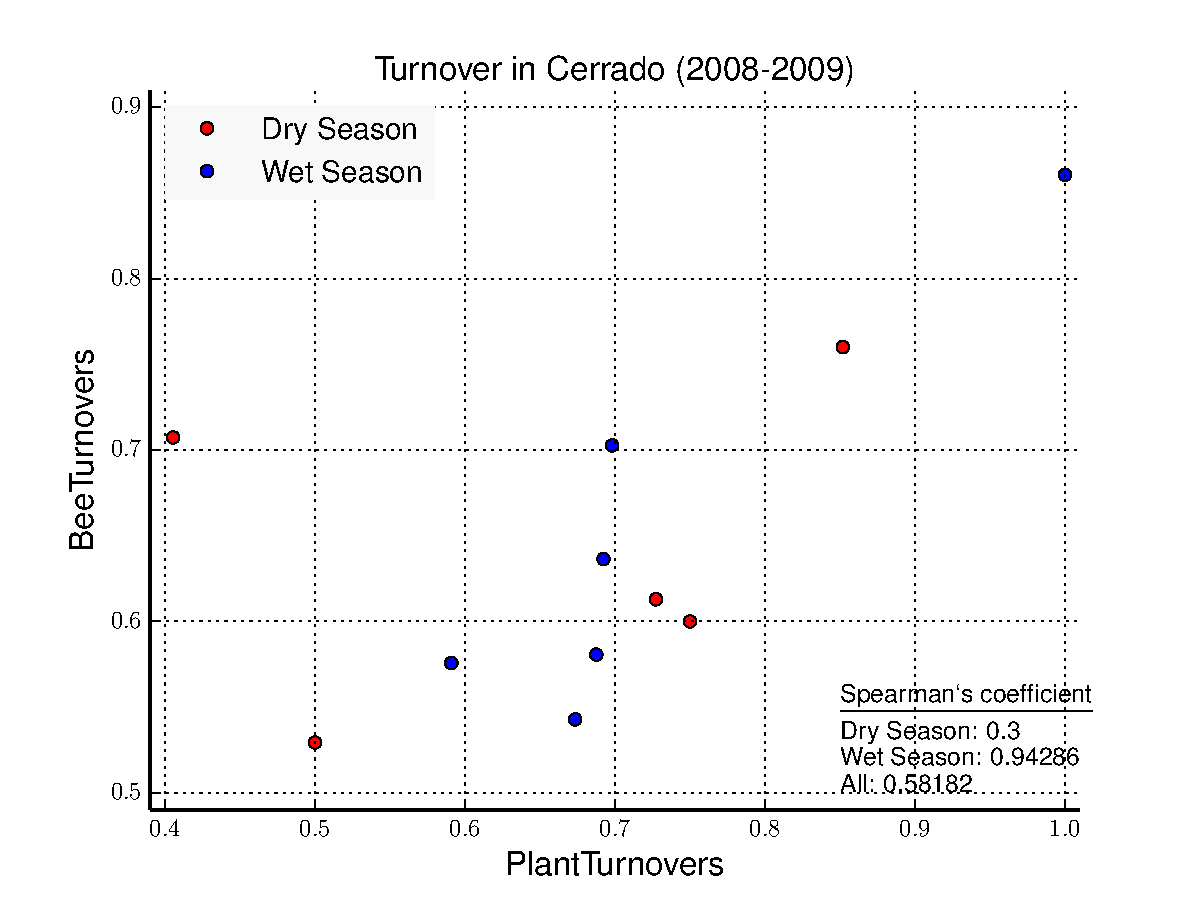
\includegraphics[width=0.48\textwidth]{PlantTurnovers-BeeTurnovers(new).pdf}%
}%\\[0.5cm] If you want some vertical space
  \label{fig:plant-bee}
\end{figure}

\newpage
\underline{Bbee or Bplant drives Bs} \\
seems to be both \\

\begin{figure}[H]
\makebox[\textwidth]{%
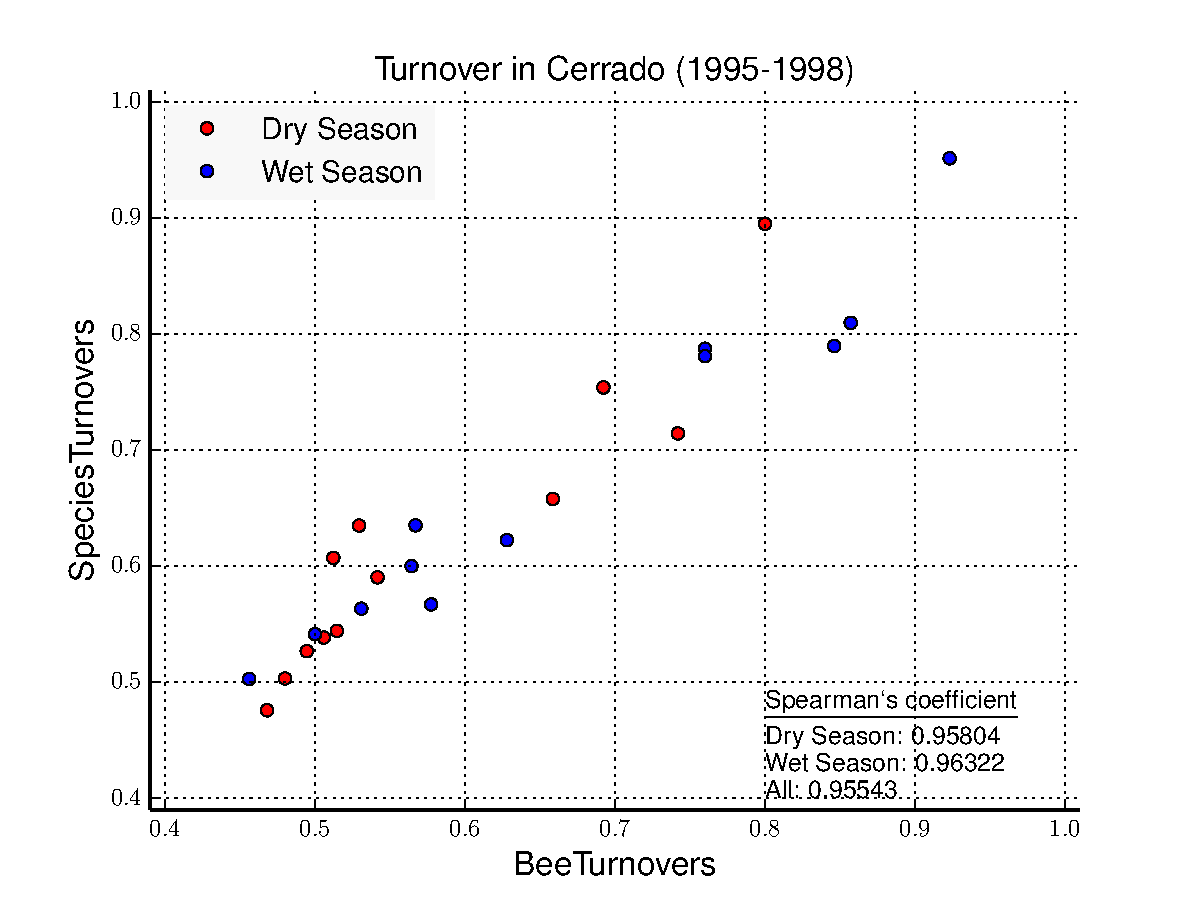
\includegraphics[width=0.48\textwidth]{BeeTurnovers-SpeciesTurnovers(old).pdf}%
\hfill    
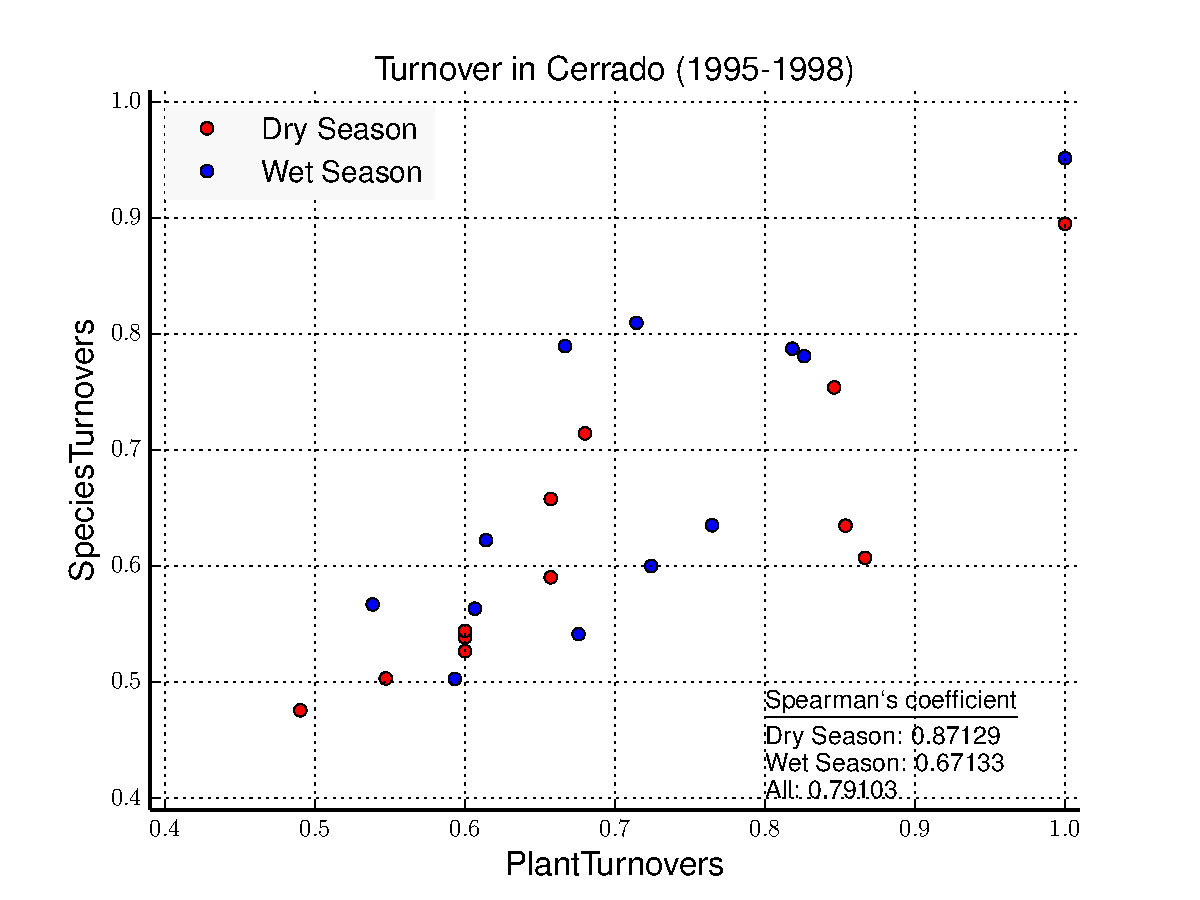
\includegraphics[width=0.48\textwidth]{PlantTurnovers-SpeciesTurnovers(old).pdf}%
}%\\[0.5cm] If you want some vertical space
  \label{fig:plant-bee}
\end{figure}

\begin{figure}[H]
\makebox[\textwidth]{%
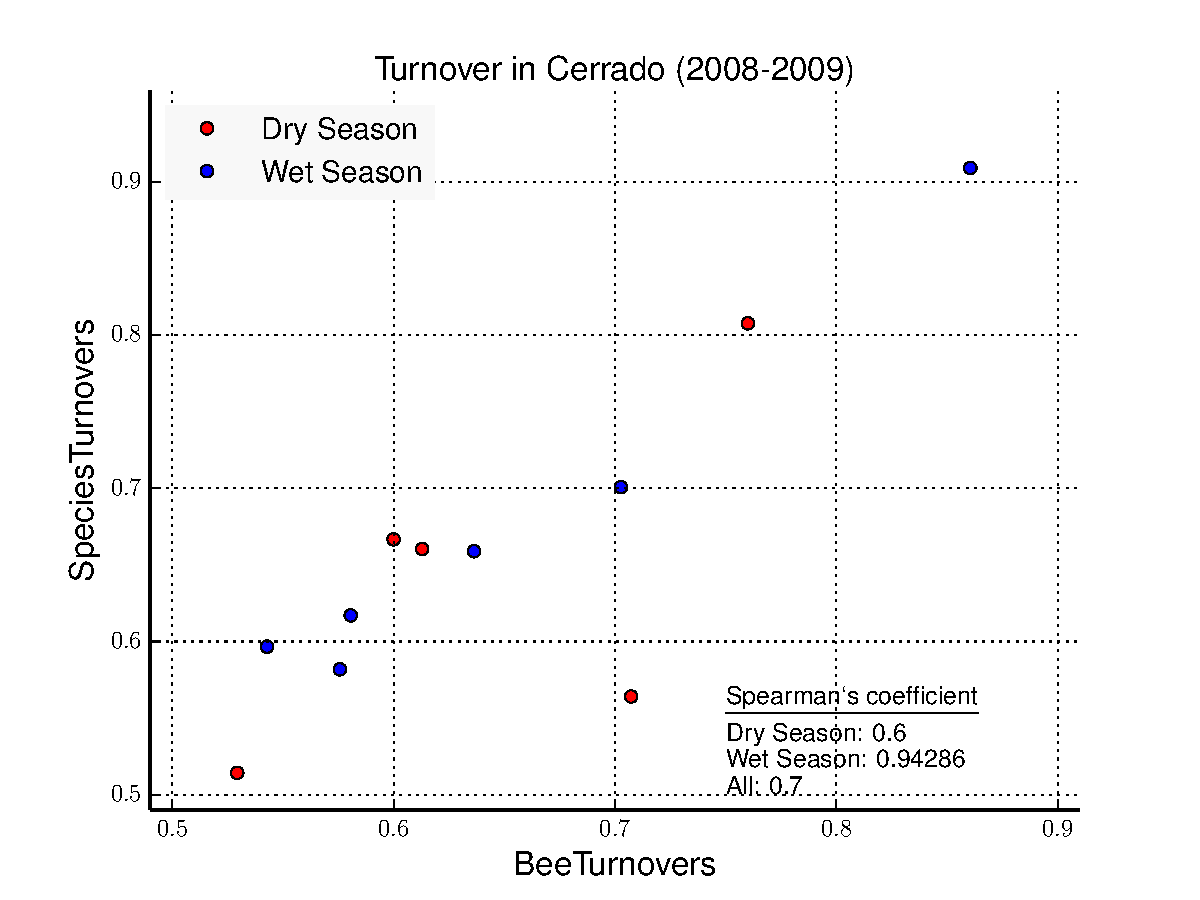
\includegraphics[width=0.48\textwidth]{BeeTurnovers-SpeciesTurnovers(new).pdf}%
\hfill    
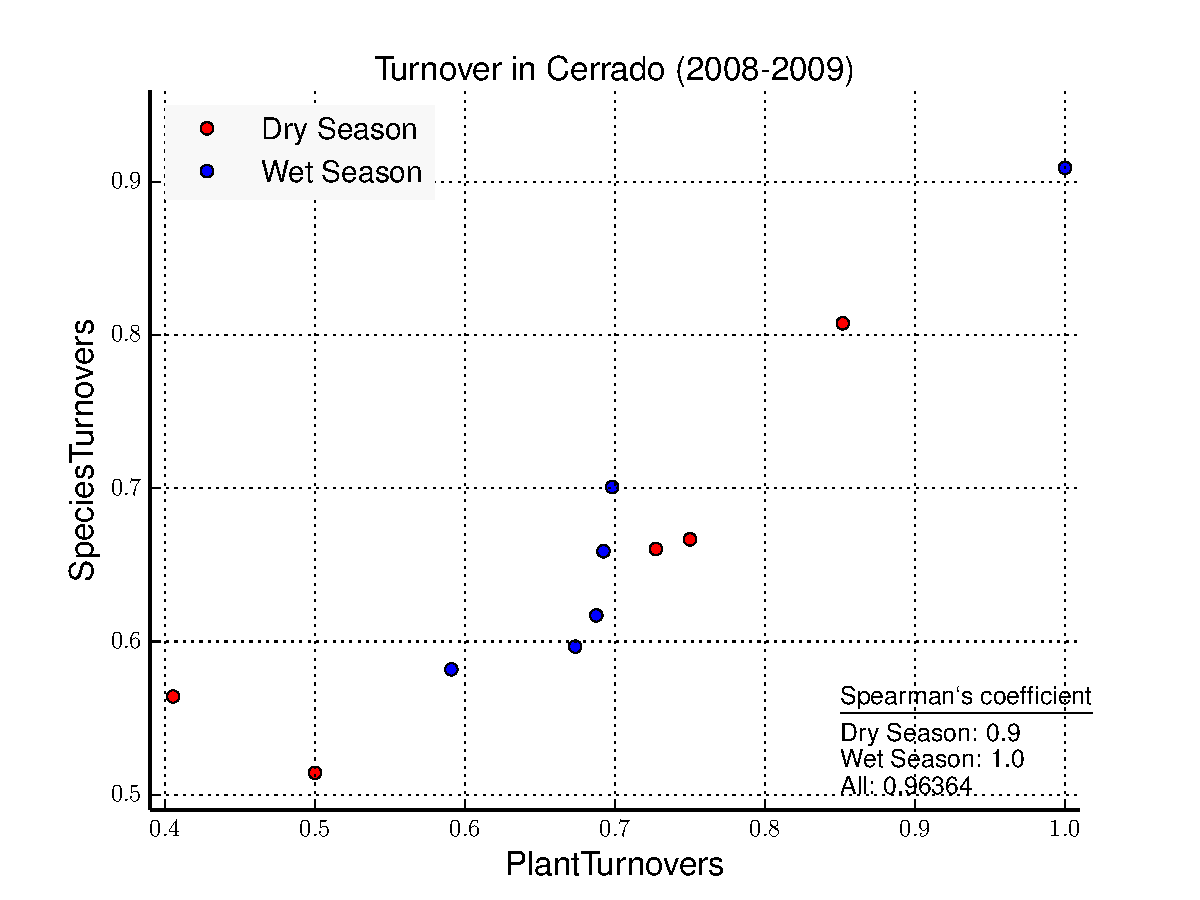
\includegraphics[width=0.48\textwidth]{PlantTurnovers-SpeciesTurnovers(new).pdf}%
}%\\[0.5cm] If you want some vertical space
  \label{fig:plant-bee}
\end{figure}

\underline{As expected, no clear pattern linking Bs to Bos} \\
Interaction rewiring driven by factors different from those driving species turnover. \\
\begin{figure}[H]
\makebox[\textwidth]{%
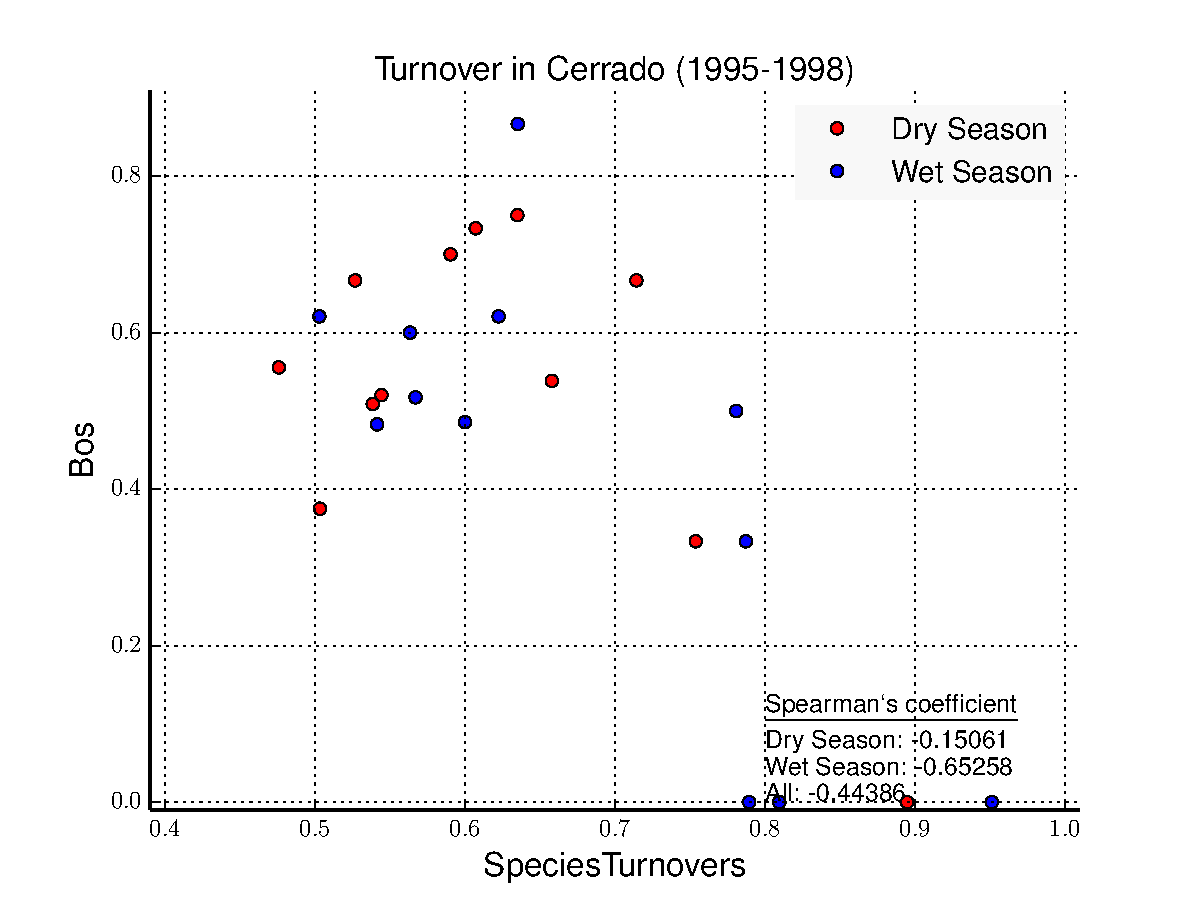
\includegraphics[width=0.48\textwidth]{SpeciesTurnovers-Bos(old).pdf}%
\hfill    
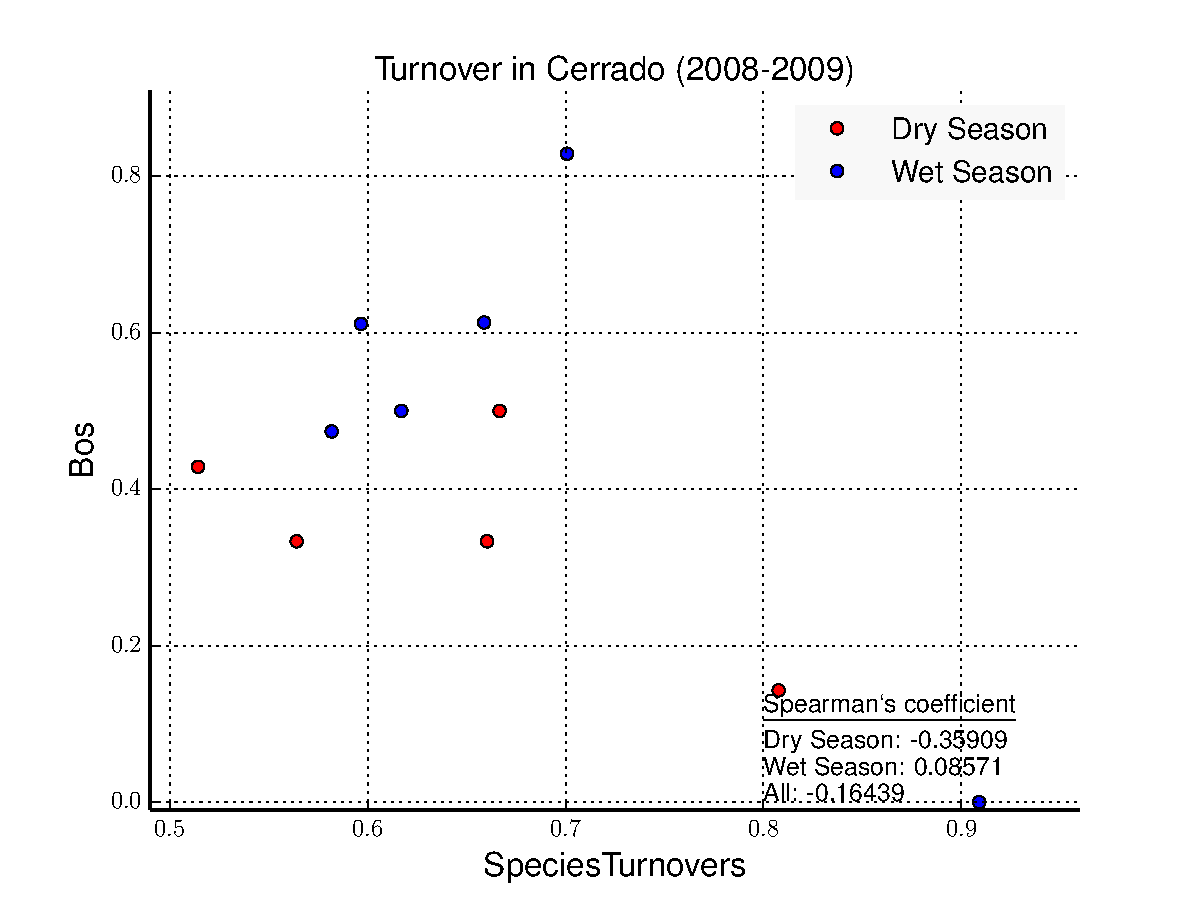
\includegraphics[width=0.48\textwidth]{SpeciesTurnovers-Bos(new).pdf}%
}%\\[0.5cm] If you want some vertical space
  \label{fig:plant-bee}
\end{figure}

\newpage
\underline{As expected, Bs correlates with Bst \& Bint} \\
\begin{figure}[H]
\makebox[\textwidth]{%
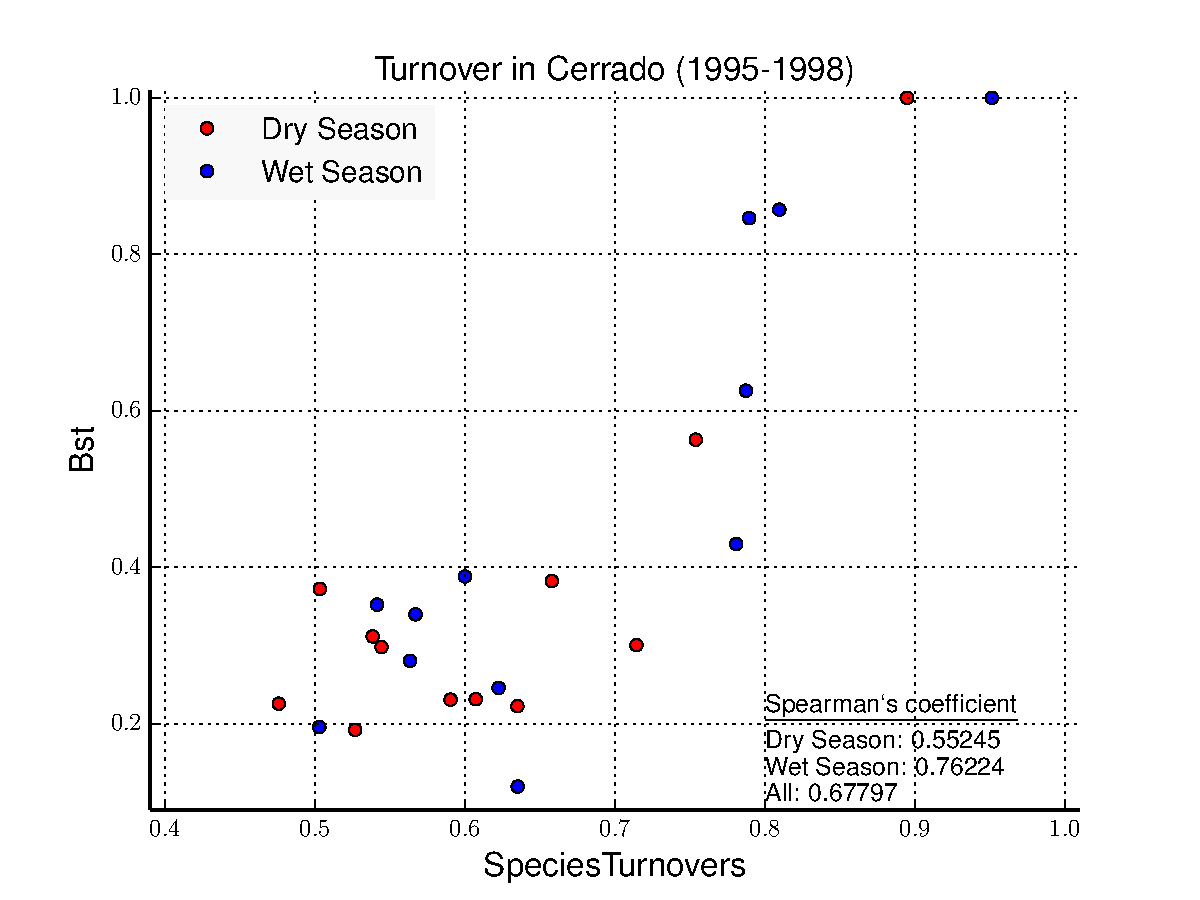
\includegraphics[width=0.48\textwidth]{SpeciesTurnovers-Bst(old).pdf}%
\hfill    
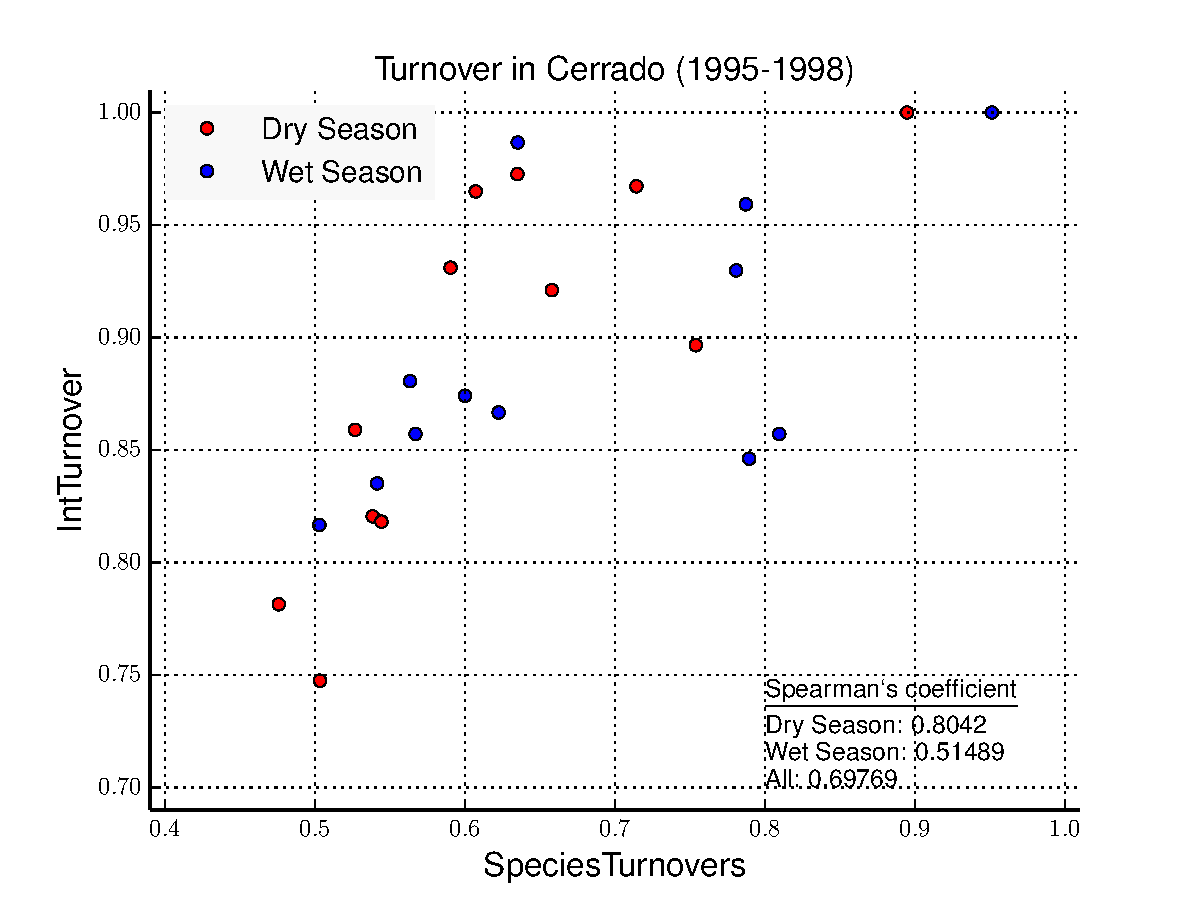
\includegraphics[width=0.48\textwidth]{SpeciesTurnovers-IntTurnover(old).pdf}%
}%\\[0.5cm] If you want some vertical space
  \label{fig:plant-bee}
\end{figure}

\begin{figure}[H]
\makebox[\textwidth]{%
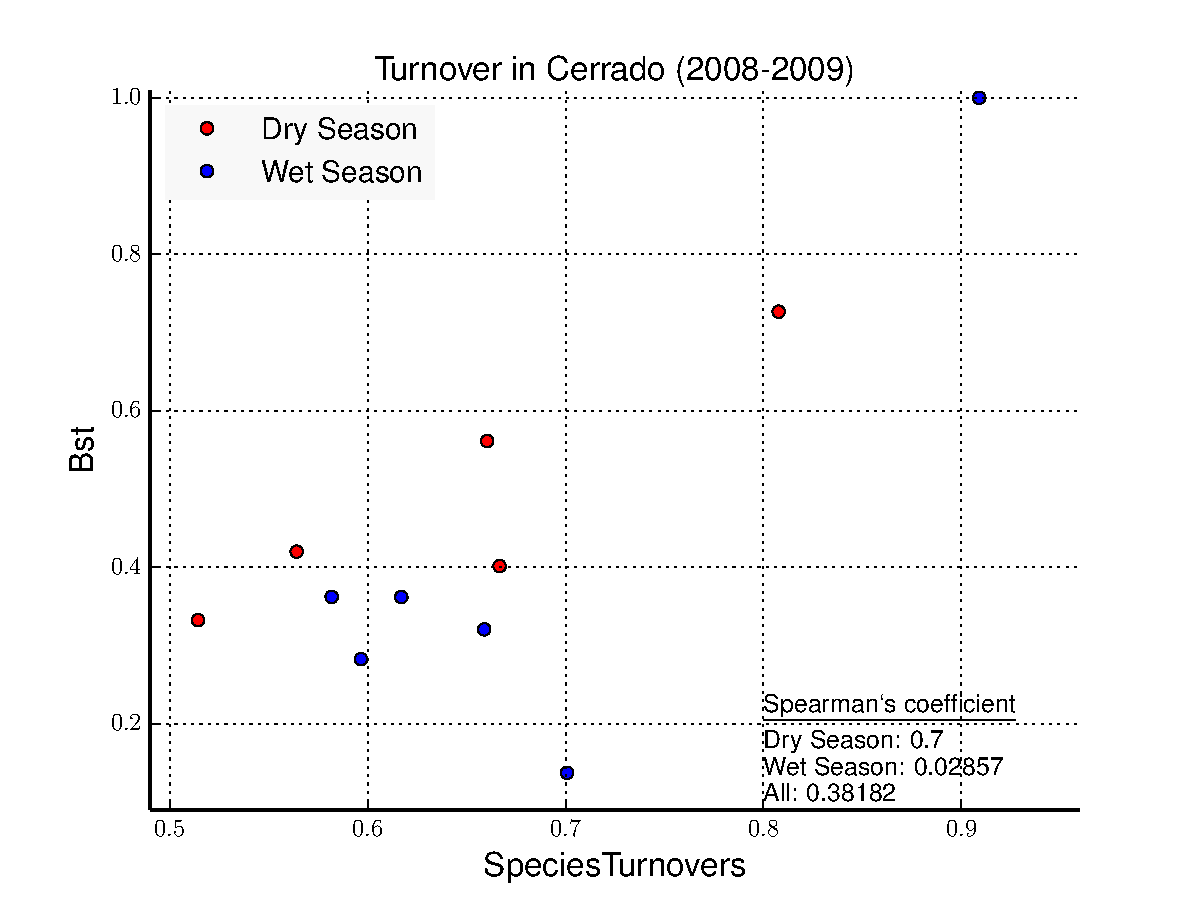
\includegraphics[width=0.48\textwidth]{SpeciesTurnovers-Bst(new).pdf}%
\hfill    
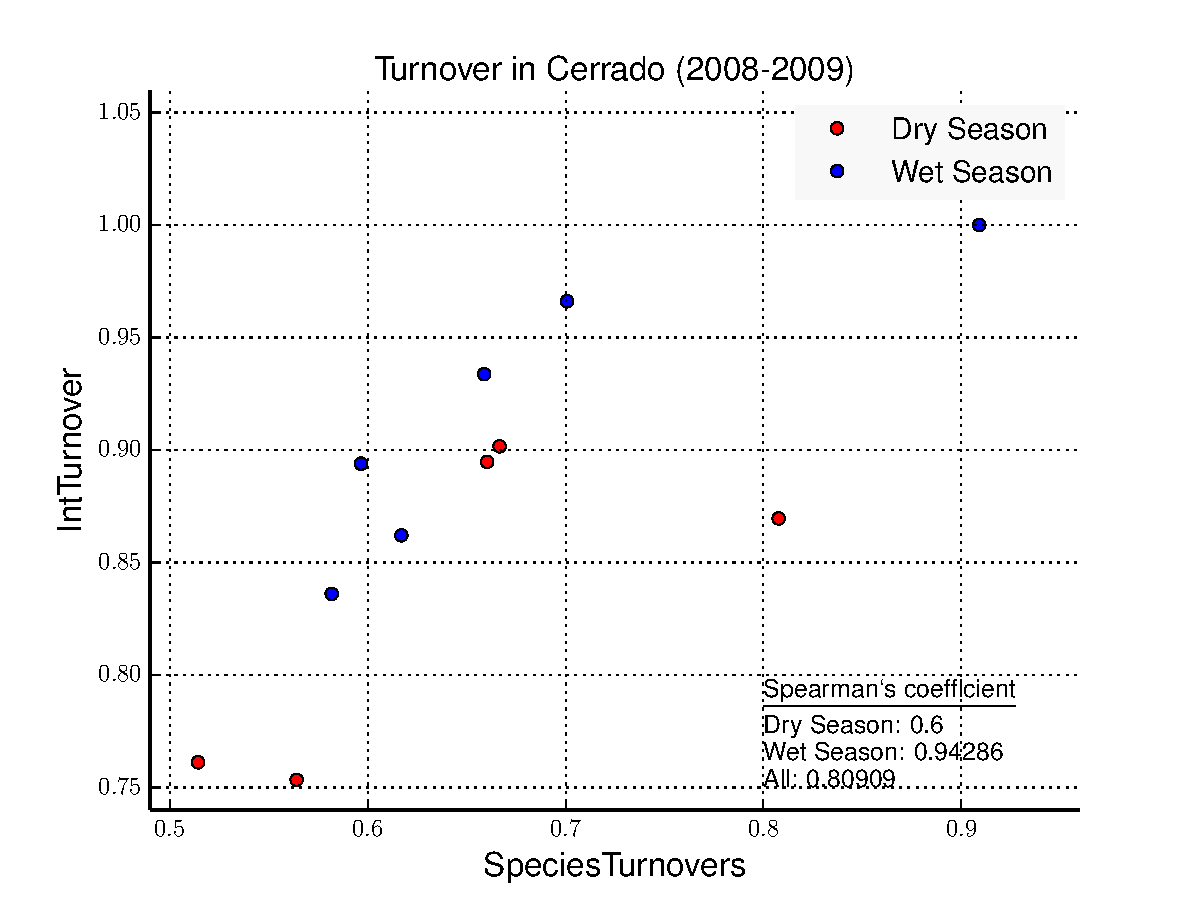
\includegraphics[width=0.48\textwidth]{SpeciesTurnovers-IntTurnover(new).pdf}%
}%\\[0.5cm] If you want some vertical space
  \label{fig:plant-bee}
\end{figure}

\subsection{climate and turnovers}
\underline{Difference in Climate between months and Average Climate between months show different patterns}\\ \autoref{fig:climate1} \autoref{fig:climate2} Refer to supplementary figures of trends across time \\
Different measures, different variables/drivers\\
do i have to do correlation or just refer to supplementary? \\
clarify the two different models \\ 

\newpage
\underline{Which model is better?} \\
Bplant, Bbee and Bos correlate better with climate diff or climate Avg \\
model fitting \\

%\begin{figure}[H]
%  \centering
%    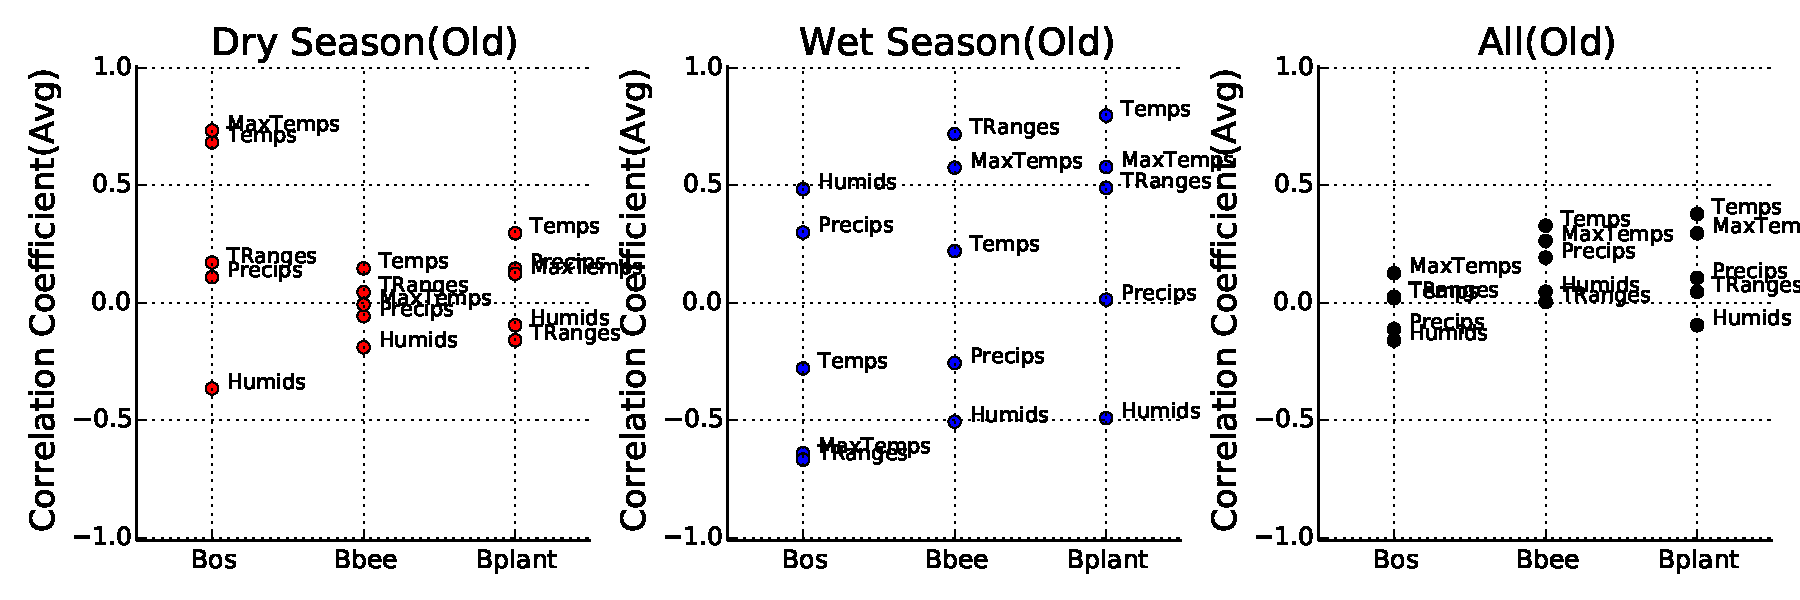
\includegraphics[width=\textwidth]{SpecTurnover&AvgClimate(Old).pdf}
%\end{figure}
%
%\begin{figure}[H]
%  \centering
%    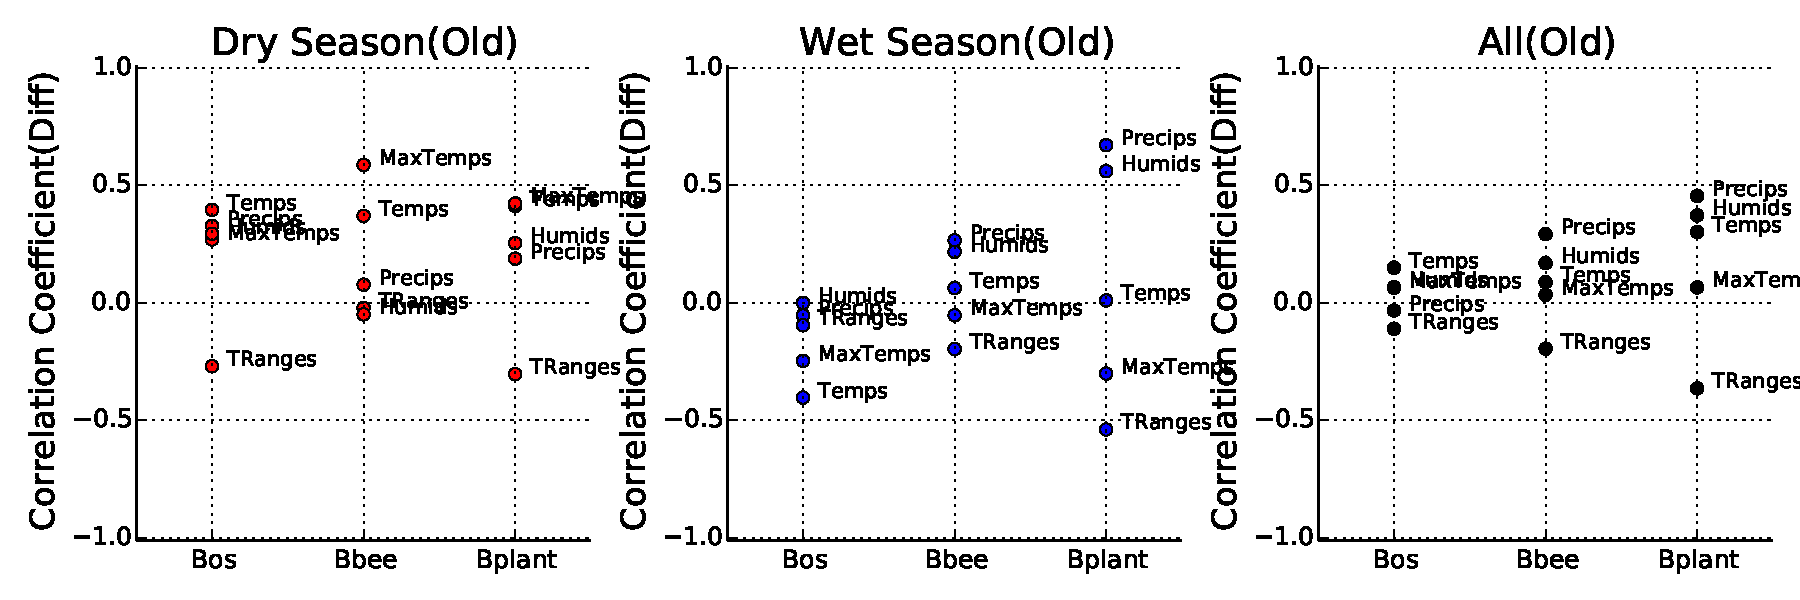
\includegraphics[width=\textwidth]{SpecTurnover&DiffClimate(Old).pdf}
%\end{figure}
%
%\newpage
%\begin{figure}[H]
%  \centering
%    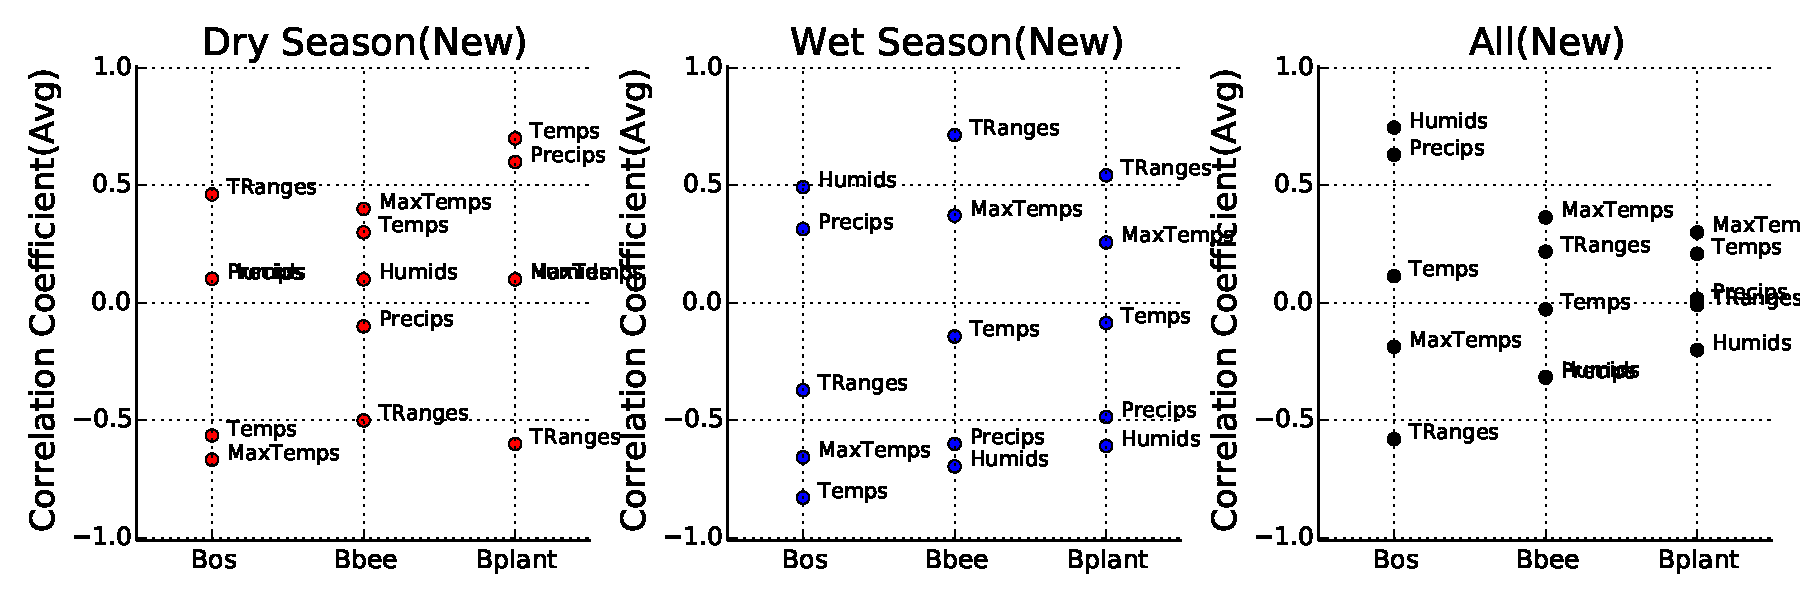
\includegraphics[width=\textwidth]{SpecTurnover&AvgClimate(New).pdf}
%\end{figure}
%
%\begin{figure}[H]
%  \centering
%    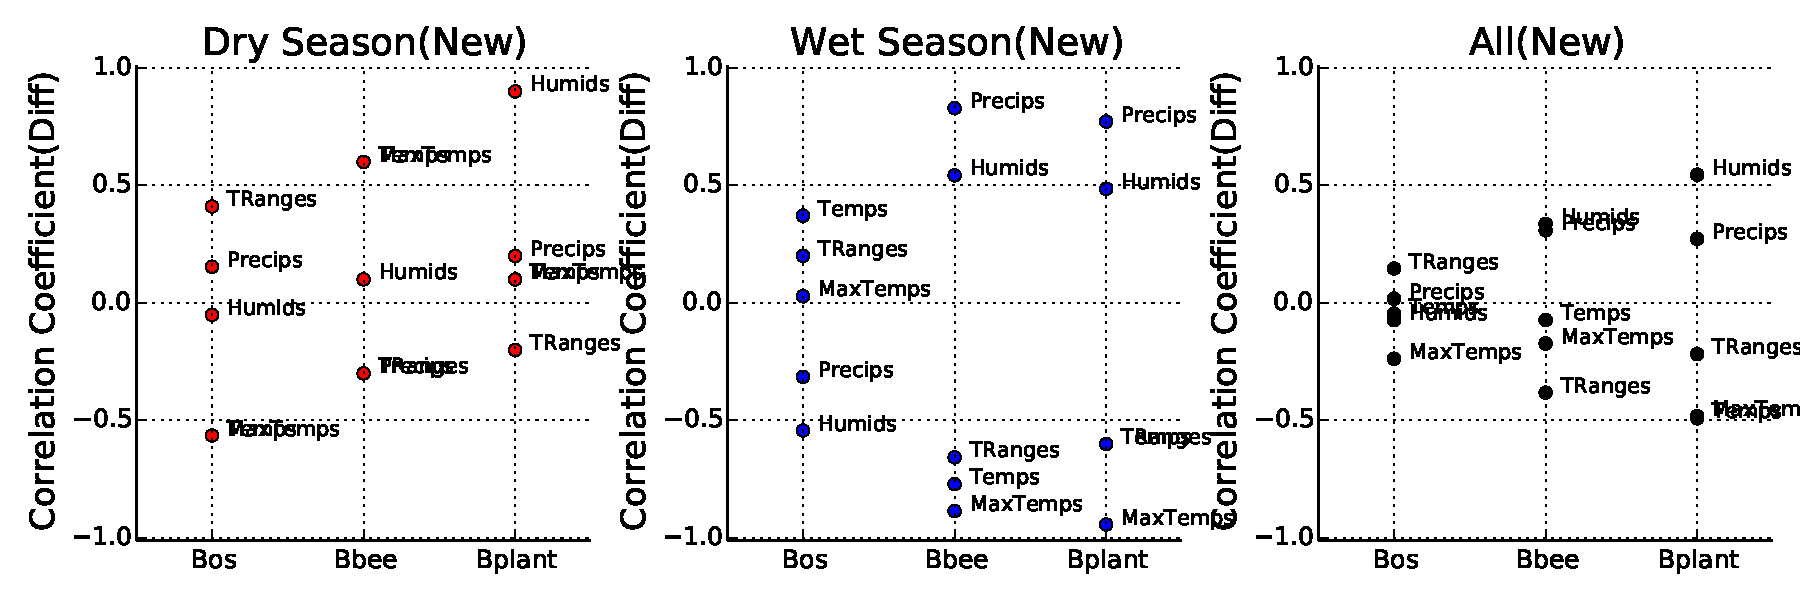
\includegraphics[width=\textwidth]{SpecTurnover&DiffClimate(New).pdf}
%\end{figure}


\begin{figure}[H]
\makebox[\textwidth]{%
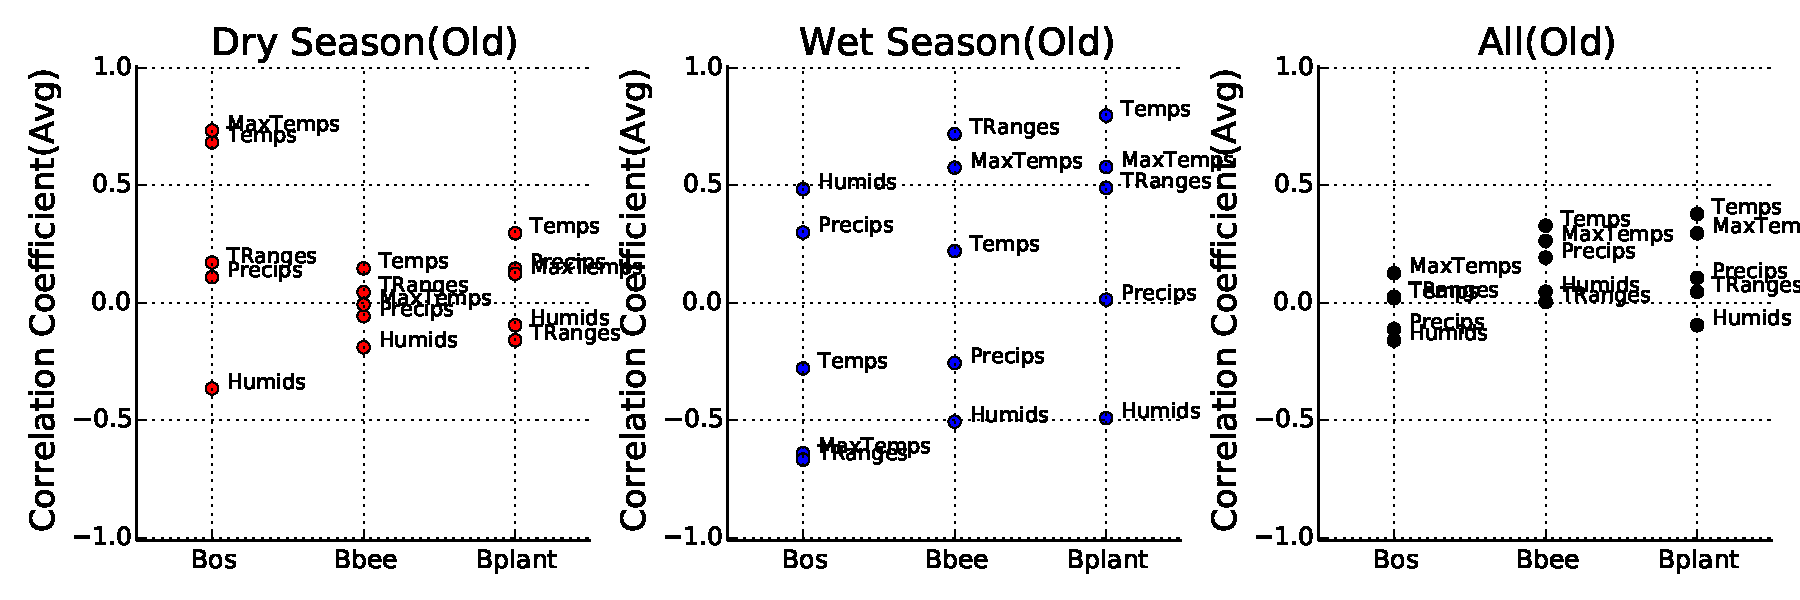
\includegraphics[width=0.50\textwidth]{SpecTurnover&AvgClimate(Old).pdf}%
\hfill    
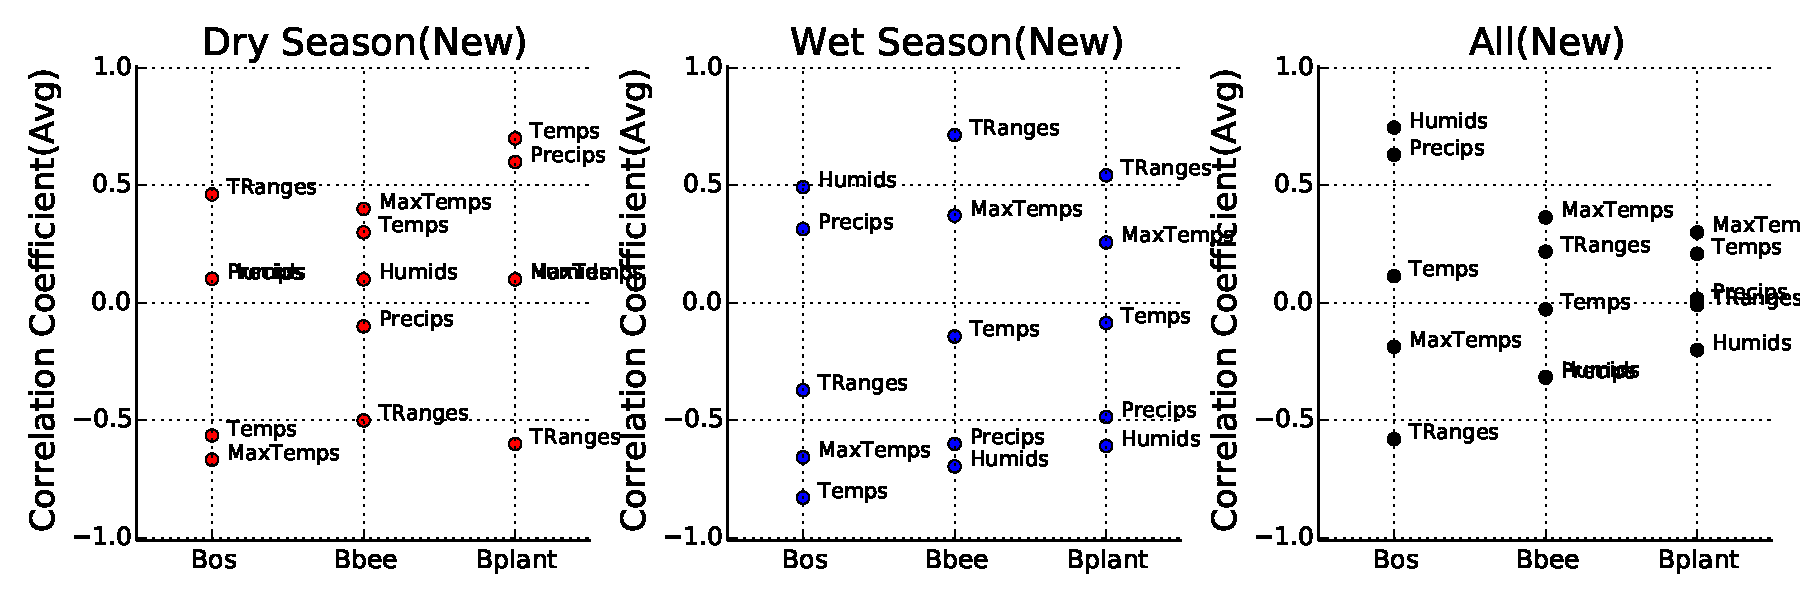
\includegraphics[width=0.50\textwidth]{SpecTurnover&AvgClimate(New).pdf}%
}%\\[0.5cm] If you want some vertical space
  \label{fig:plant-bee}
\end{figure}

\begin{figure}[H]
\makebox[\textwidth]{%
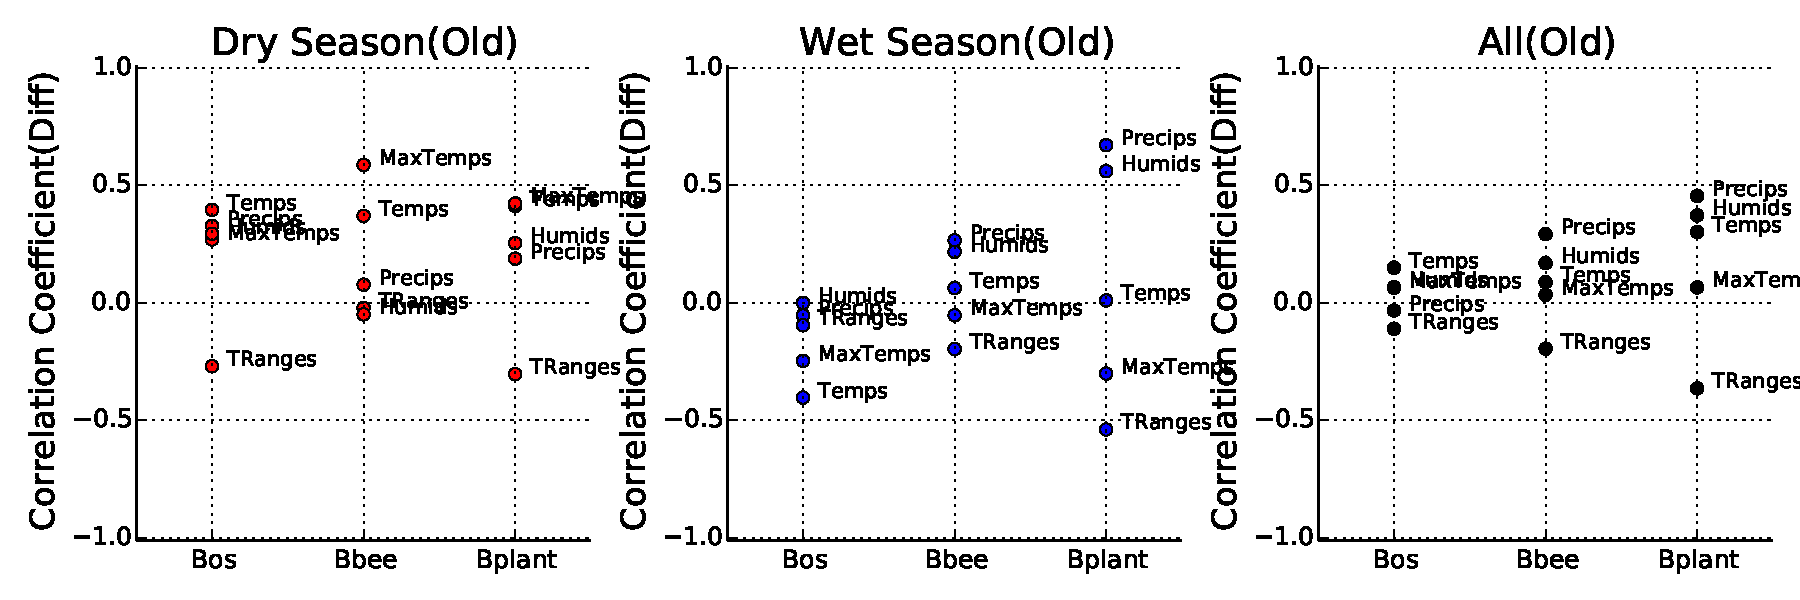
\includegraphics[width=0.50\textwidth]{SpecTurnover&DiffClimate(Old).pdf}%
\hfill    
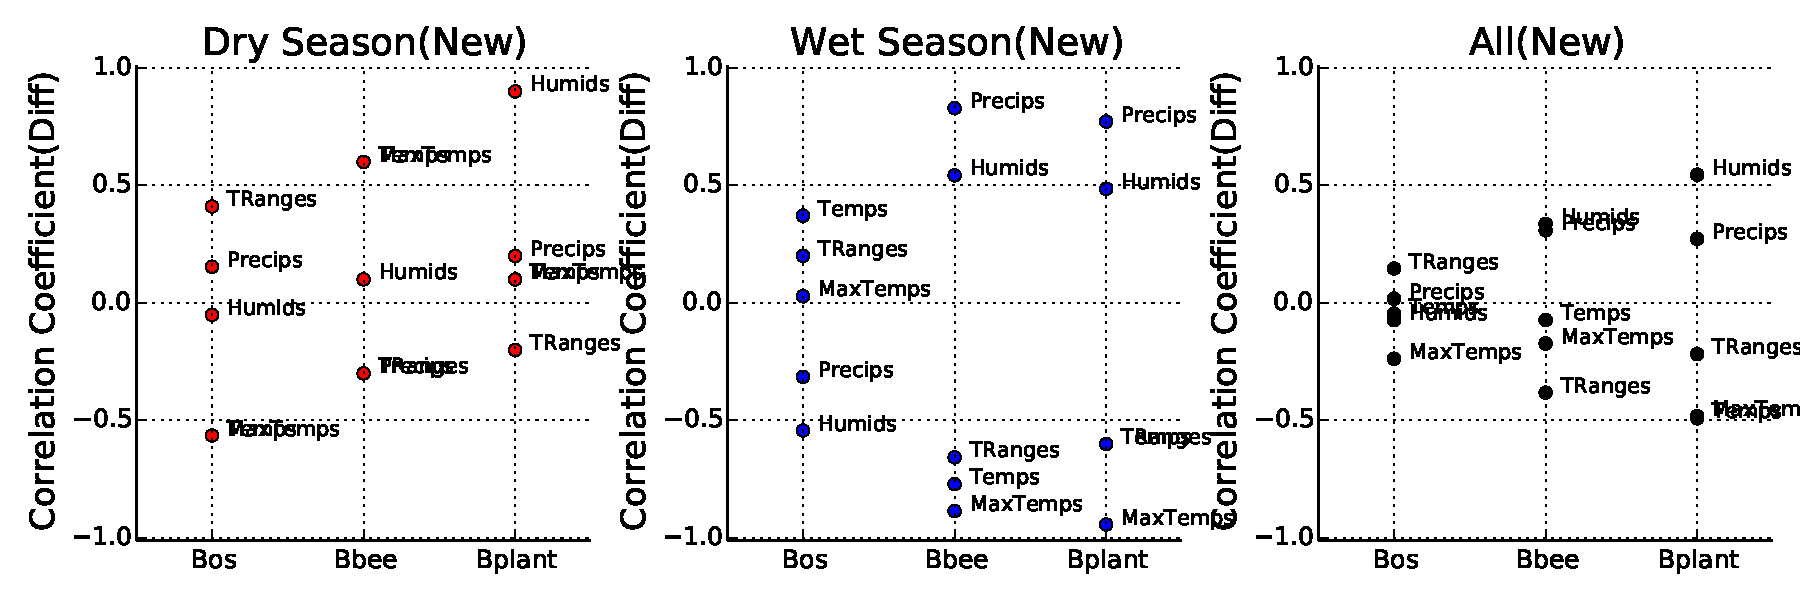
\includegraphics[width=0.50\textwidth]{SpecTurnover&DiffClimate(New).pdf}%
}%\\[0.5cm] If you want some vertical space
  \label{fig:plant-bee}
\end{figure}

\underline{Which climatic factor best for Bplant, Bbee and Bos} \\

\underline{Climatic factor best for Bplant and Bbee, same for Bs and Bst} \\

\underline{diff climate factor for Bos vs Bst? } \\

\underline{Can we use a climatic factor as predictor for Bint?} \\

\newpage
\section{Discussion} % 1800 words
Discuss results, why climatic factor would explain turnover \\
Limitations: Correlation does not relate to causation, but diff to conduct such experiments,  \\
Future Research: more data, artic temperature comparisons \\

\section*{Supplementary Data}
spearman test p-value \& monte carlo p-values \\
add poster figure, how B-diversity is calculated example  \\
all networks \\
correlation plots \\
all turnover values \\
all correlation values \\

\newpage
\begin{landscape}

\begin{figure}[H]
  \centering
    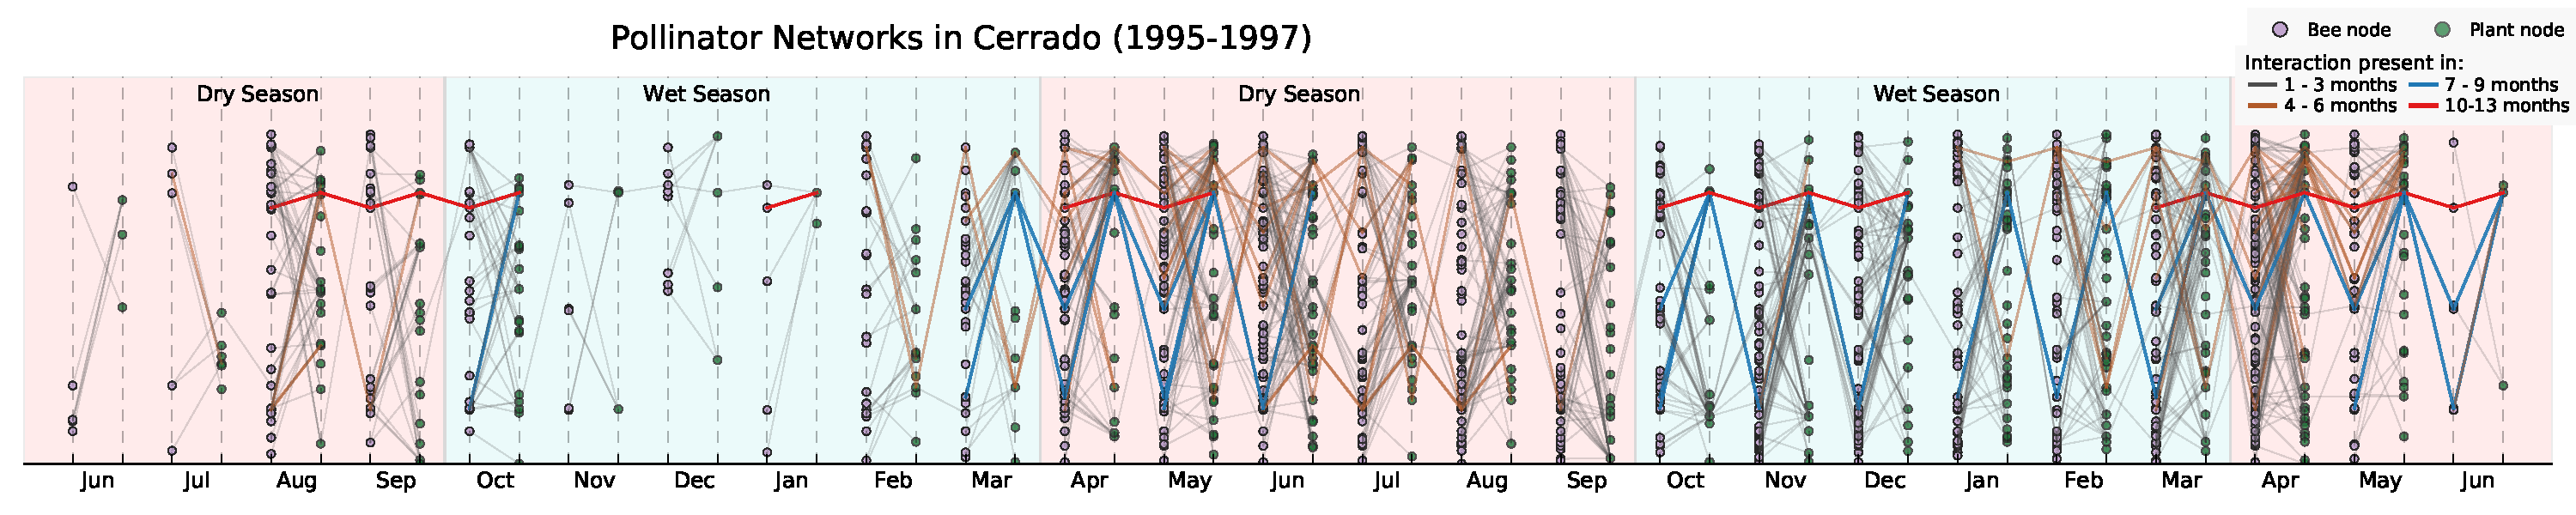
\includegraphics[width=260mm]{network(old).pdf}
\end{figure}

\begin{figure}[H]
  \centering
    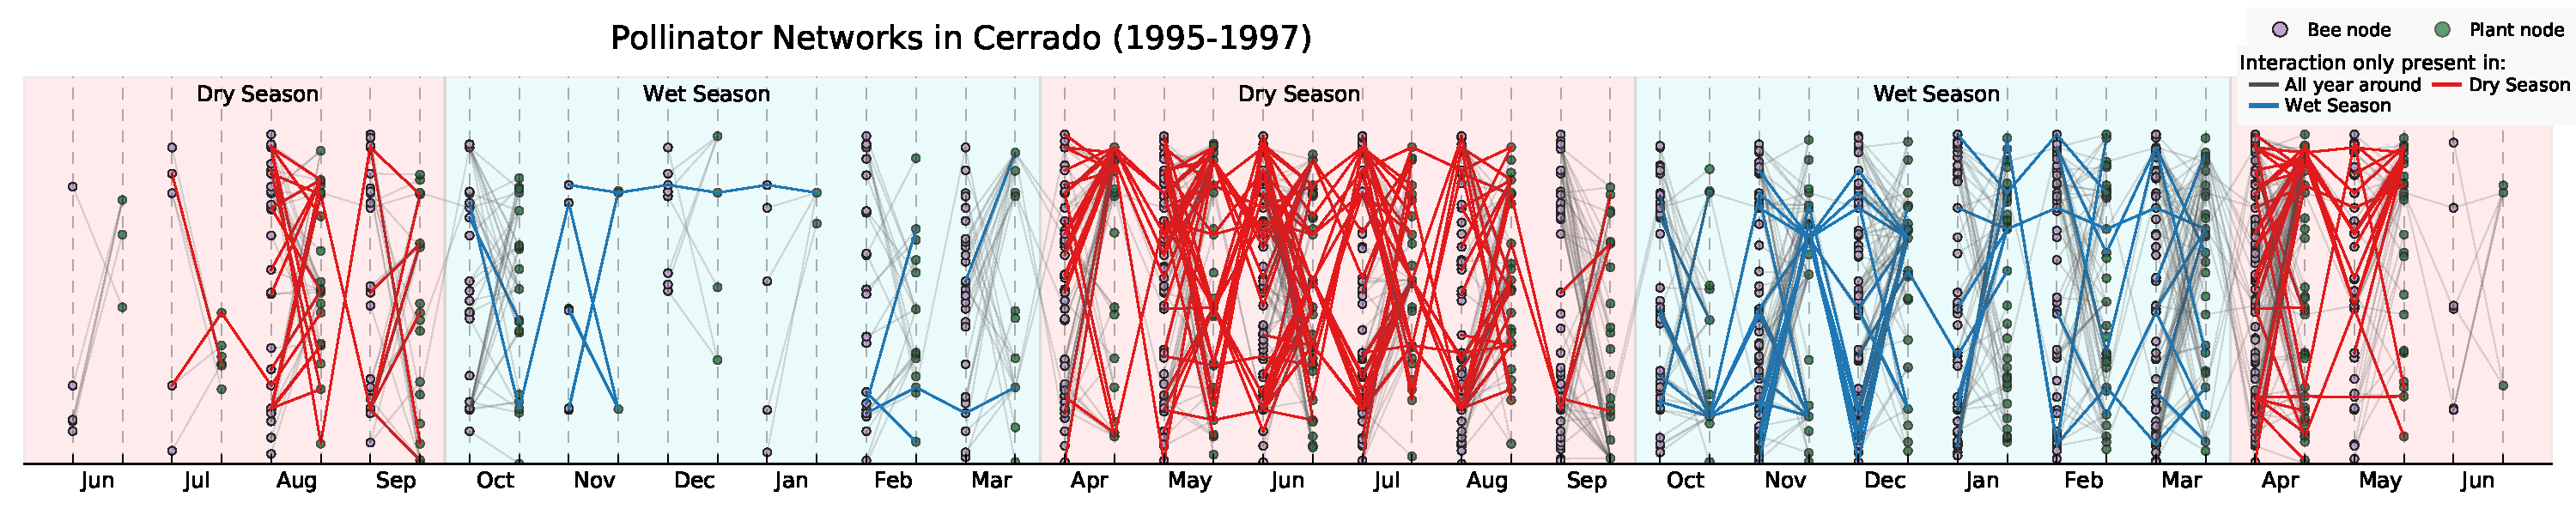
\includegraphics[width=260mm]{seasonalnetwork(old).pdf}
\end{figure}

\begin{figure}[H]
  \centering
    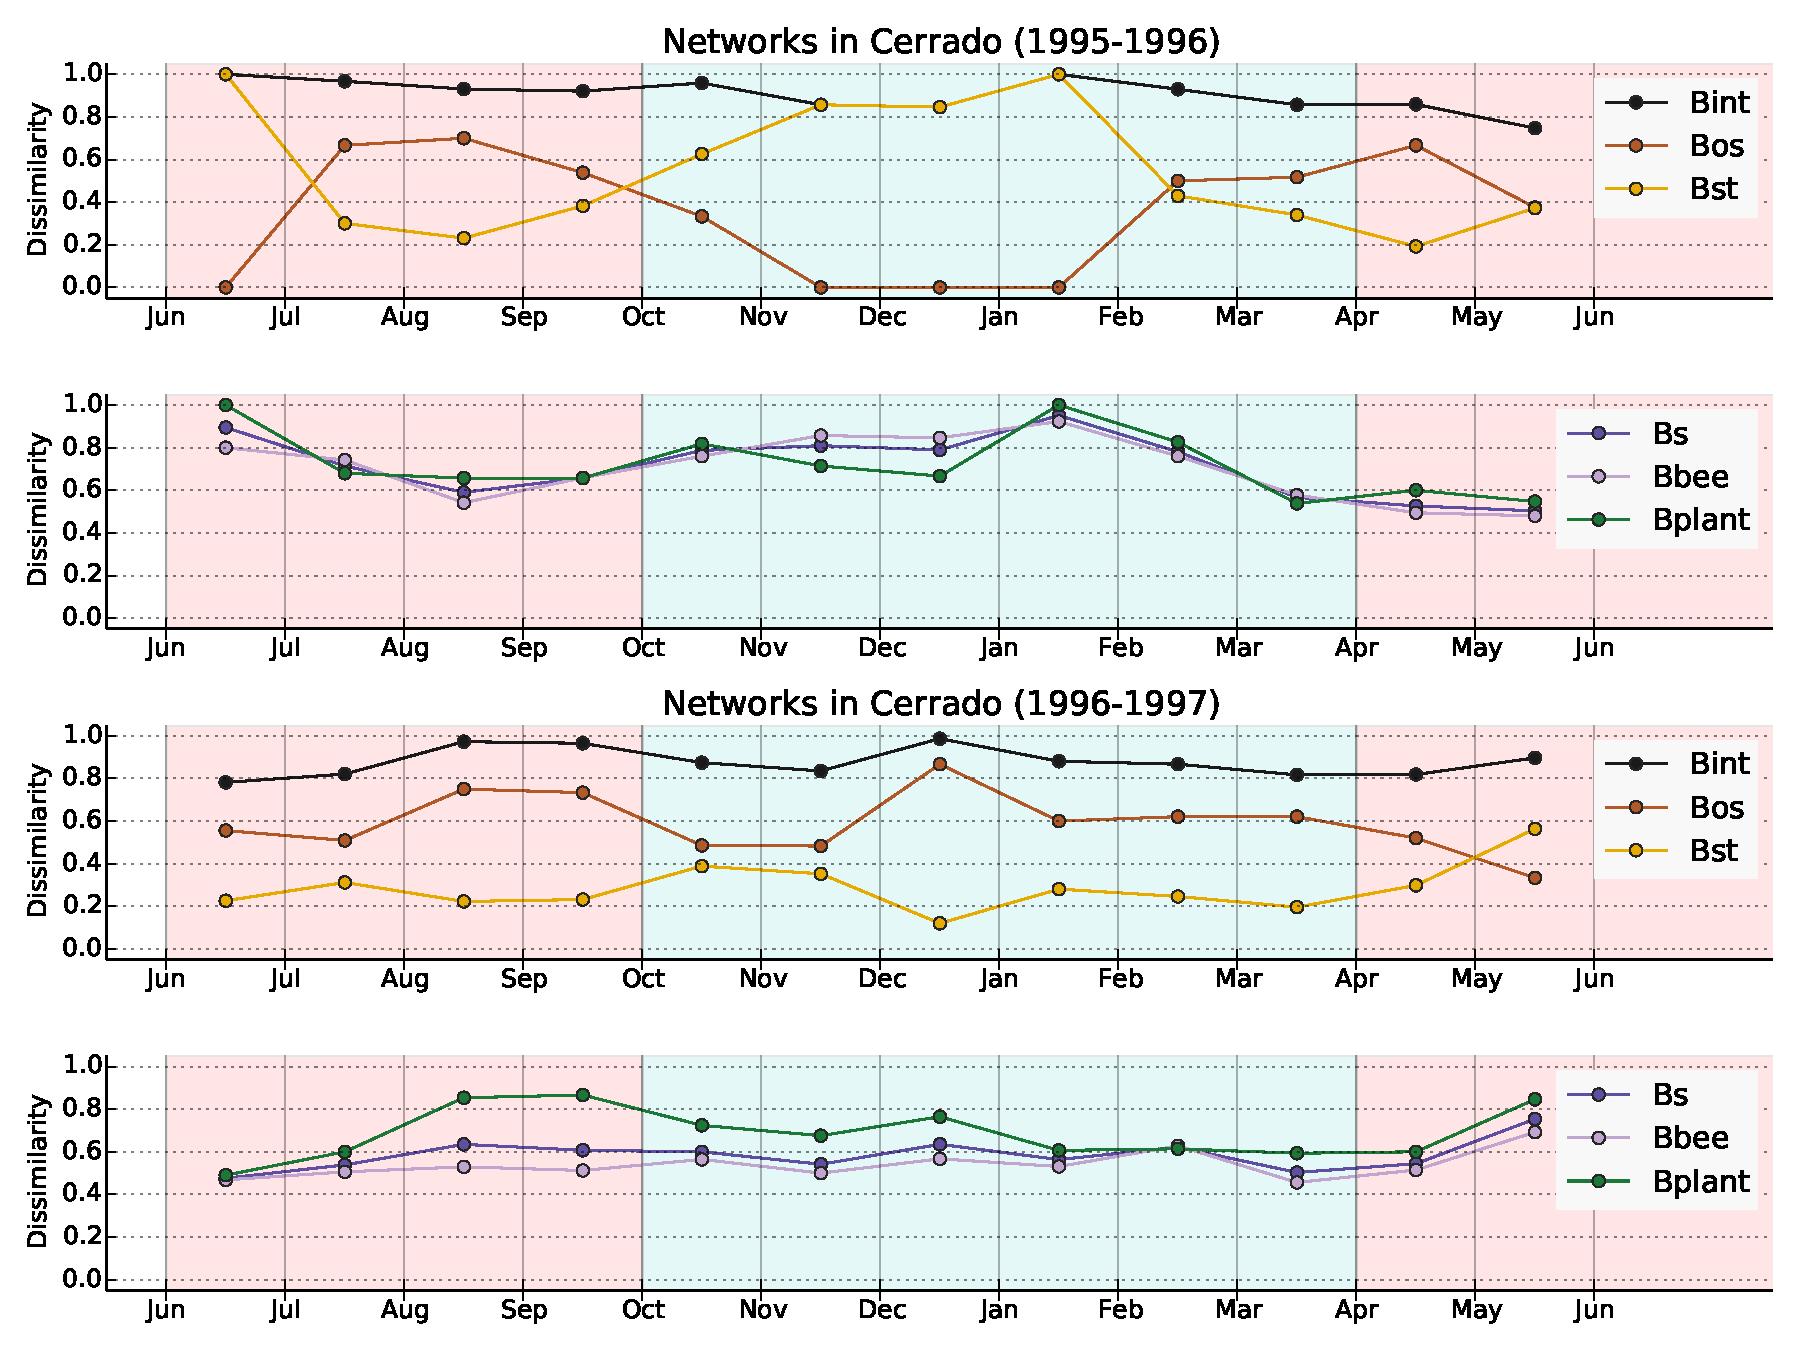
\includegraphics[width=250mm]{TurnoversAcrossTime(old).pdf}
\end{figure}

\begin{figure}[H]
  \centering
    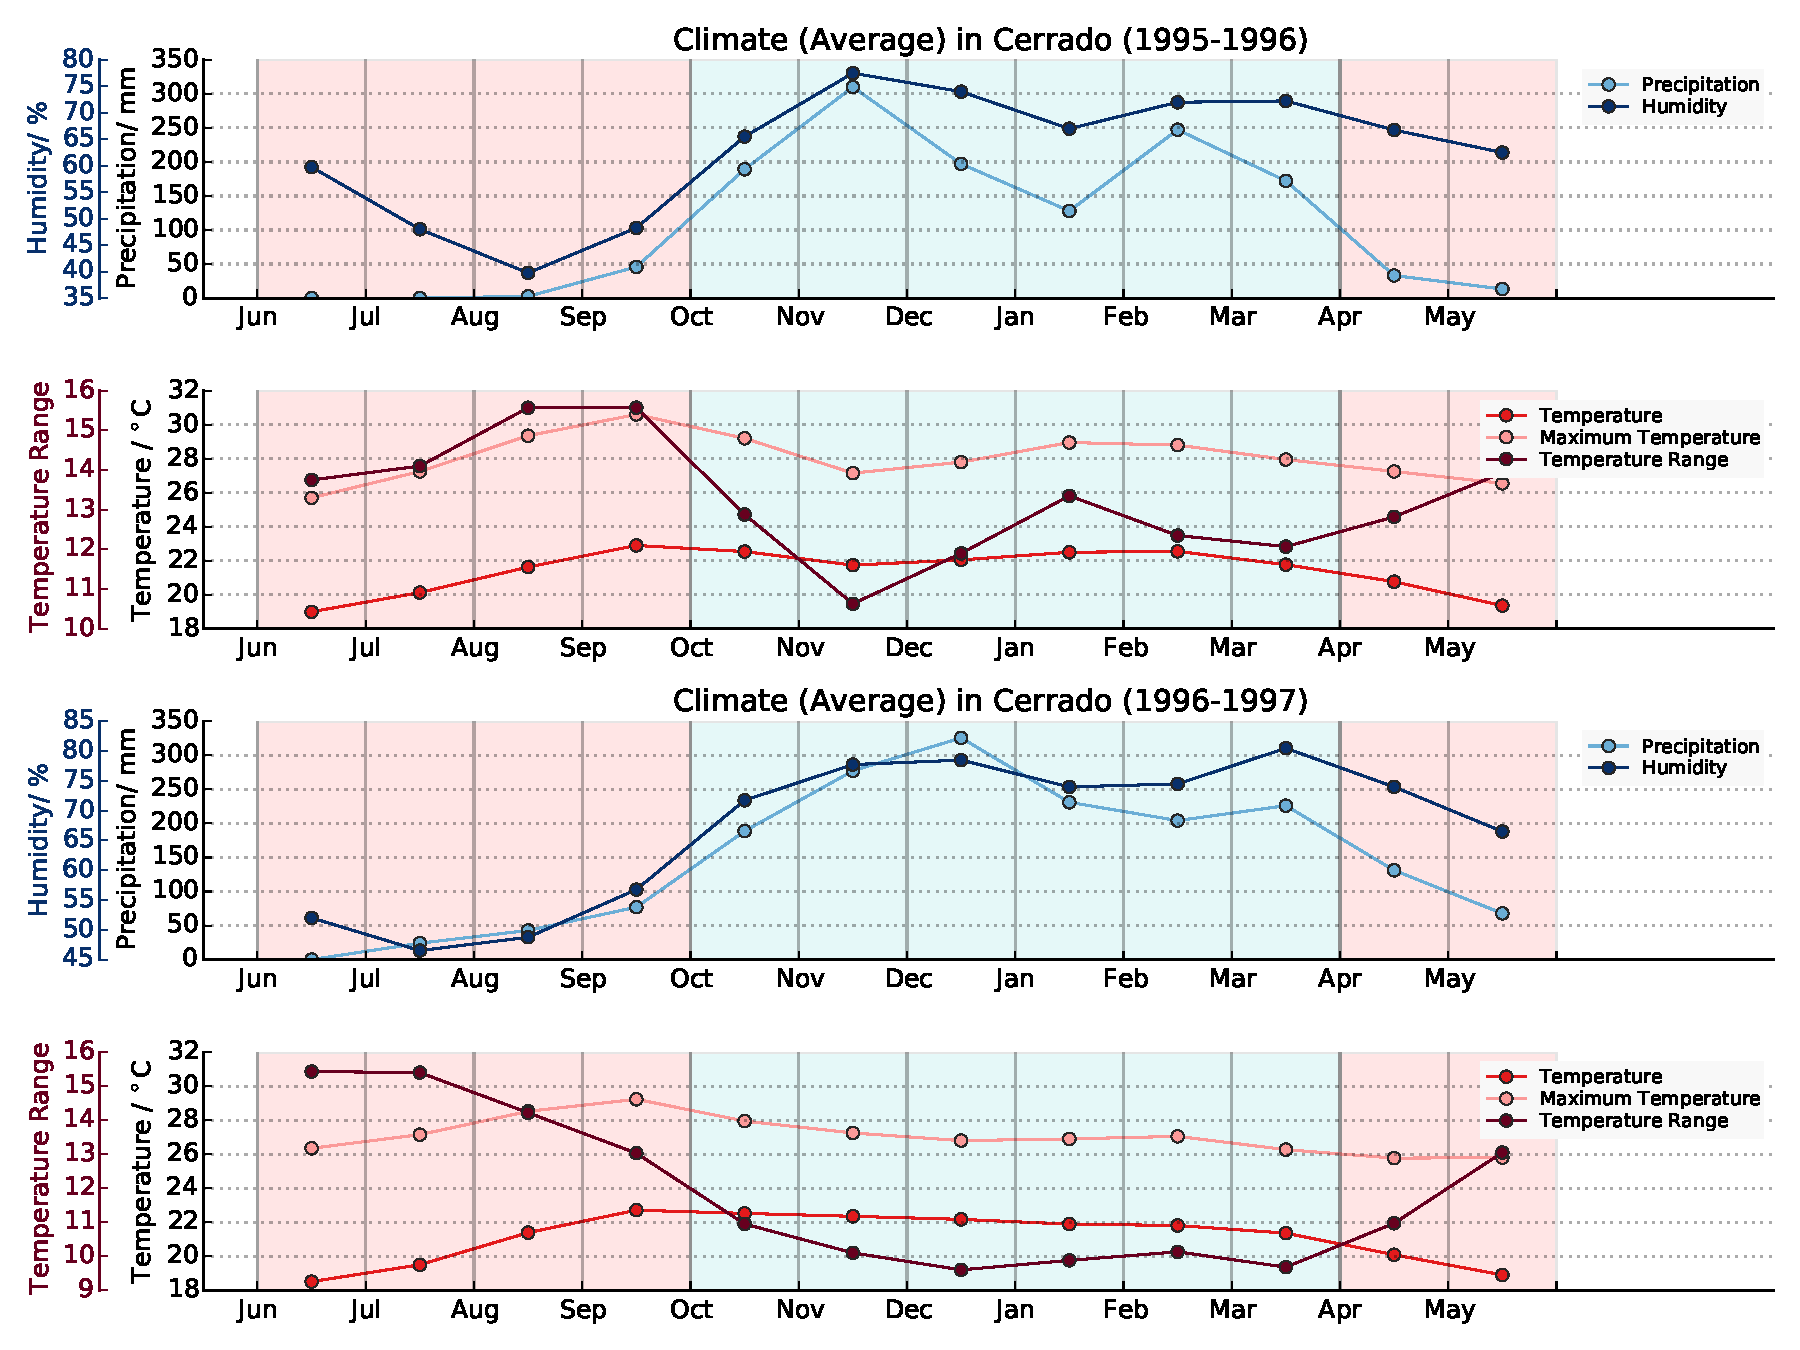
\includegraphics[width=250mm]{AvgClimateAcrossTime(Old).pdf}
    \label{fig:climate1}
\end{figure}

\begin{figure}[H]
  \centering
    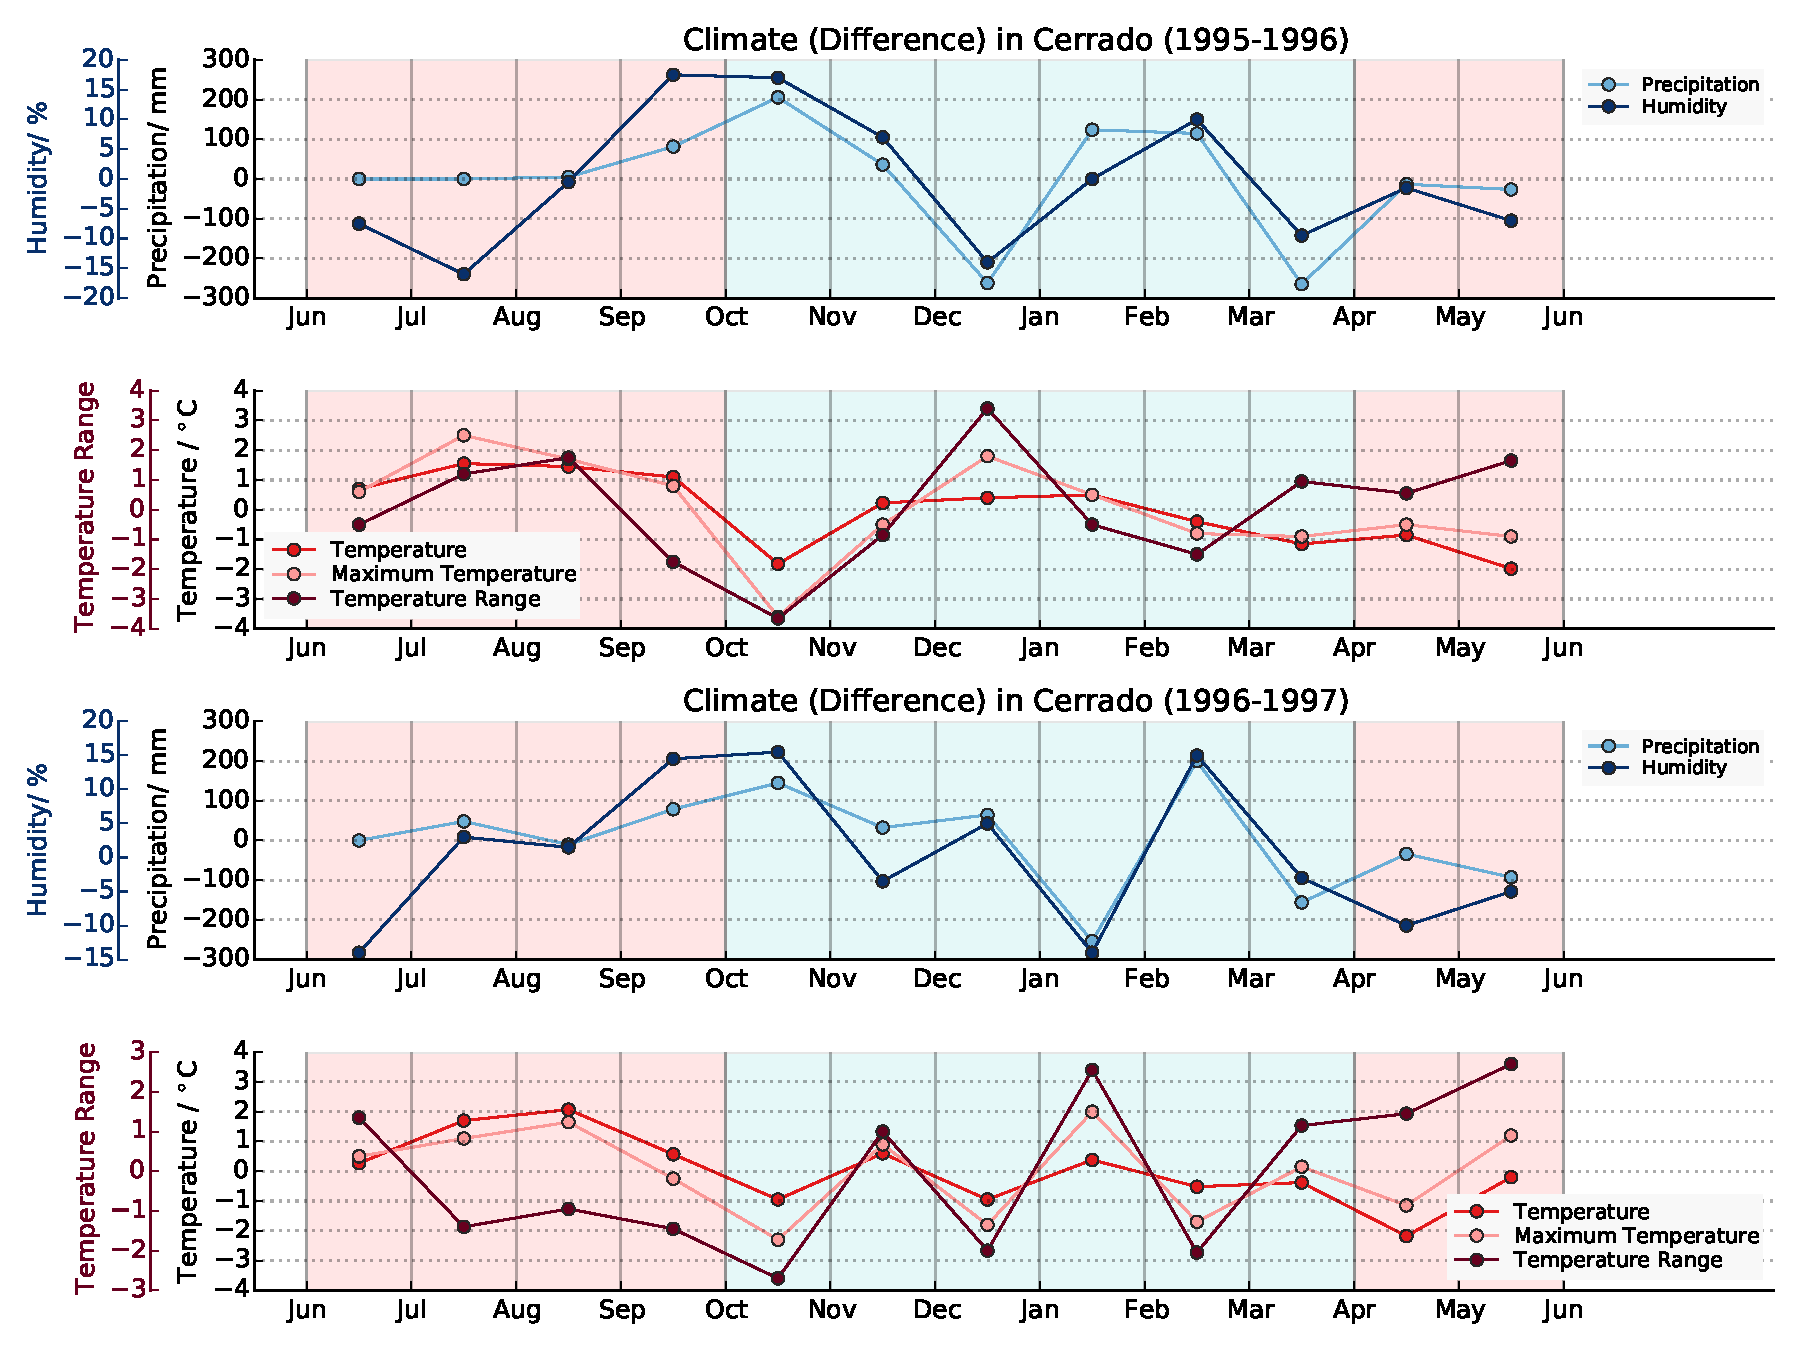
\includegraphics[width=250mm]{DiffClimateAcrossTime(Old).pdf}
\end{figure}

\begin{figure}[H]
  \centering
    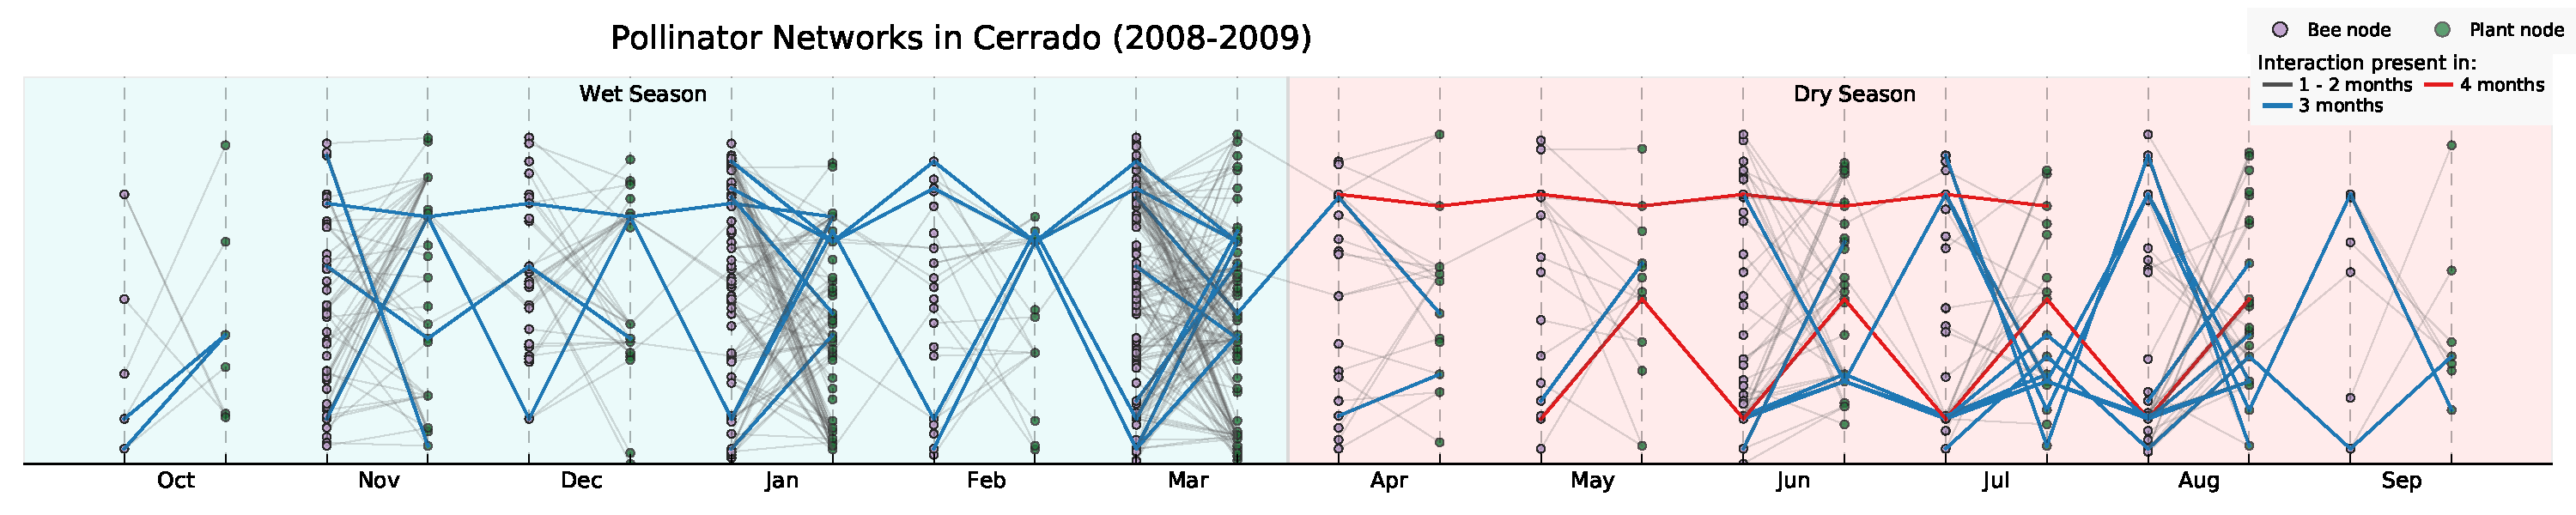
\includegraphics[width=255mm]{network(new).pdf}
\end{figure}

\begin{figure}[H]
  \centering
    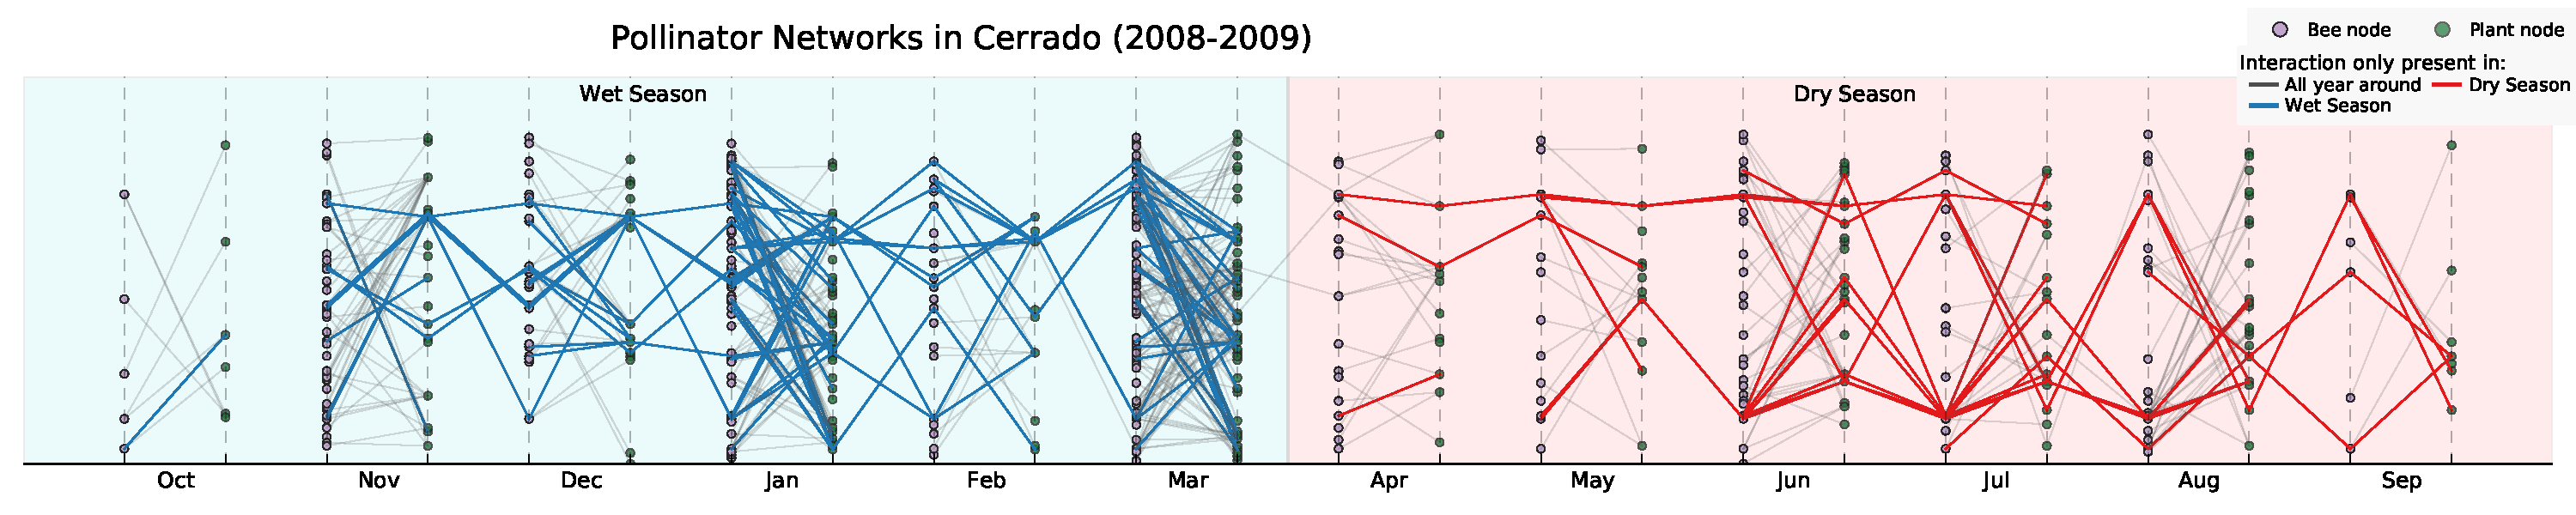
\includegraphics[width=255mm]{seasonalnetwork(new).pdf}
\end{figure}

\begin{figure}[H]
  \centering
    \includegraphics[width=250mm]{TurnoversAcrossTime(new).pdf}
\end{figure}

\begin{figure}[H]
  \centering
    \includegraphics[width=250mm]{ClimateAcrossTime(new).pdf}
    \label{fig:climate2}
\end{figure}
\end{landscape}

\newpage
\bibliography{BEEquations}
\bibliographystyle{cell}

\end{document}


